% ================= IF YOU HAVE QUESTIONS =======================
%
% Technical questions to bbob@lri.fr
% ===============================================================
%
\documentclass{article}
%%%%%%%%%%%%%%%%%%%%%%%%%%%%% PREAMBLE   %%%%%%%%%%%%%%%%%%%%%%%%%%%%%%%%%%%%%%
\usepackage{amssymb,amsmath}
\usepackage[dvipsnames]{xcolor}
\usepackage{xcolor}
\usepackage{float}
\usepackage{rotating}

\newcommand{\DIM}{\ensuremath{\mathrm{DIM}}}
\newcommand{\ERT}{\ensuremath{\mathrm{ERT}}}
\newcommand{\FEvals}{\ensuremath{\mathrm{FEvals}}}
\newcommand{\nruns}{\ensuremath{\mathrm{Nruns}}}
\newcommand{\Dfb}{\ensuremath{\Delta f_{\mathrm{best}}}}
\newcommand{\Df}{\ensuremath{\Delta f}}
\newcommand{\nbFEs}{\ensuremath{\mathrm{\#FEs}}}
\newcommand{\fopt}{\ensuremath{f_\mathrm{opt}}}
\newcommand{\ftarget}{\ensuremath{f_\mathrm{t}}}
\newcommand{\CrE}{\ensuremath{\mathrm{CrE}}}
\newcommand{\rot}[2][2.5]{
  \hspace*{-3.5\baselineskip}%
  \begin{rotate}{90}\hspace{#1em}#2
  \end{rotate}}
%%%%%%%%%%%%%%%%%%%%   END OF PREAMBLE   %%%%%%%%%%%%%%%%%%%%%%%%%%%%%%%%%%%%%%
% \newcommand{\bbobdatapath}{ppdata2/} % was default output folder of rungeneric2.py 
\newcommand{\bbobdatapath}{ppdata/} % default output folder of rungeneric.py
\input{\bbobdatapath bbob_pproc_commands.tex}  % \algorithmA, \algorithmB
% if necessary, redefine names for 1st algorithm (1st arg. of post-processing) and 2nd algorithm (2nd arg.) 
% \renewcommand{\algorithmA}{mynameA} % first argument in the post-processing
% \renewcommand{\algorithmB}{mynameB} % second argument in the post-processing

\graphicspath{{\bbobdatapath}}

\title{Black-Box Optimization Benchmarking Template for the Comparison of Two Algorithms on the Noiseless Testbed}
\author{}

\begin{document}

\maketitle

% \section{Introduction}
%
% \section{Algorithm Presentation}
%
% \section{Experimental Procedure}
%
%%%%%%%%%%%%%%%%%%%%%%%%%%%%%%%%%%%%%%%%%%%%%%%%%%%%%%%%%%%%%%%%%%%%%%%%%%%%%%%
\section{Results}
%%%%%%%%%%%%%%%%%%%%%%%%%%%%%%%%%%%%%%%%%%%%%%%%%%%%%%%%%%%%%%%%%%%%%%%%%%%%%%%
Results from experiments according to \cite{hansen2010exp} on the benchmark
functions given in \cite{wp200901_2010,hansen2010fun} are presented in
Figures~\ref{fig:RLDs05Da}, \ref{fig:RLDs05Db}, \ref{fig:RLDs20Db}, \ref{fig:scatterplots}, \ref{fig:ERTratiographs}, and
Tables~\ref{tab:ERTs05D} and \ref{tab:ERTs20D}.
The \textbf{expected running time (\ERT)}, used in the figures and table,
depends on a given target function value, $\ftarget=\fopt+\Df$, and is computed
over all relevant trials as the number of function evaluations executed during
each trial while the best function value did not reach \ftarget, summed over
all trials and divided by the number of trials that actually reached \ftarget\
\cite{hansen2010exp,price1997dev}.
\textbf{Statistical significance} is tested with the rank-sum test for a given
target $\Delta\ftarget$ using, for each trial, either the number of needed
function evaluations to reach $\Delta\ftarget$ (inverted and multiplied by
$-1$), or, if the target was not reached, the best $\Df$-value achieved,
measured only up to the smallest number of overall function evaluations for any
unsuccessful trial under consideration if available.
%The description of figures and tables is given in \cite{}.
%%%%%%%%%%%%%%%%%%%%%%%%%%%%%%%%%%%%%%%%%%%%%%%%%%%%%%%%%%%%%%%%%%%%%%%%%%%%%%%
%%%%%%%%%%%%%%%%%%%%%%%%%%%%%%%%%%%%%%%%%%%%%%%%%%%%%%%%%%%%%%%%%%%%%%%%%%%%%%%
\begin{figure}
\centering
\begin{tabular}{@{}c@{}c@{}c@{}c@{}}
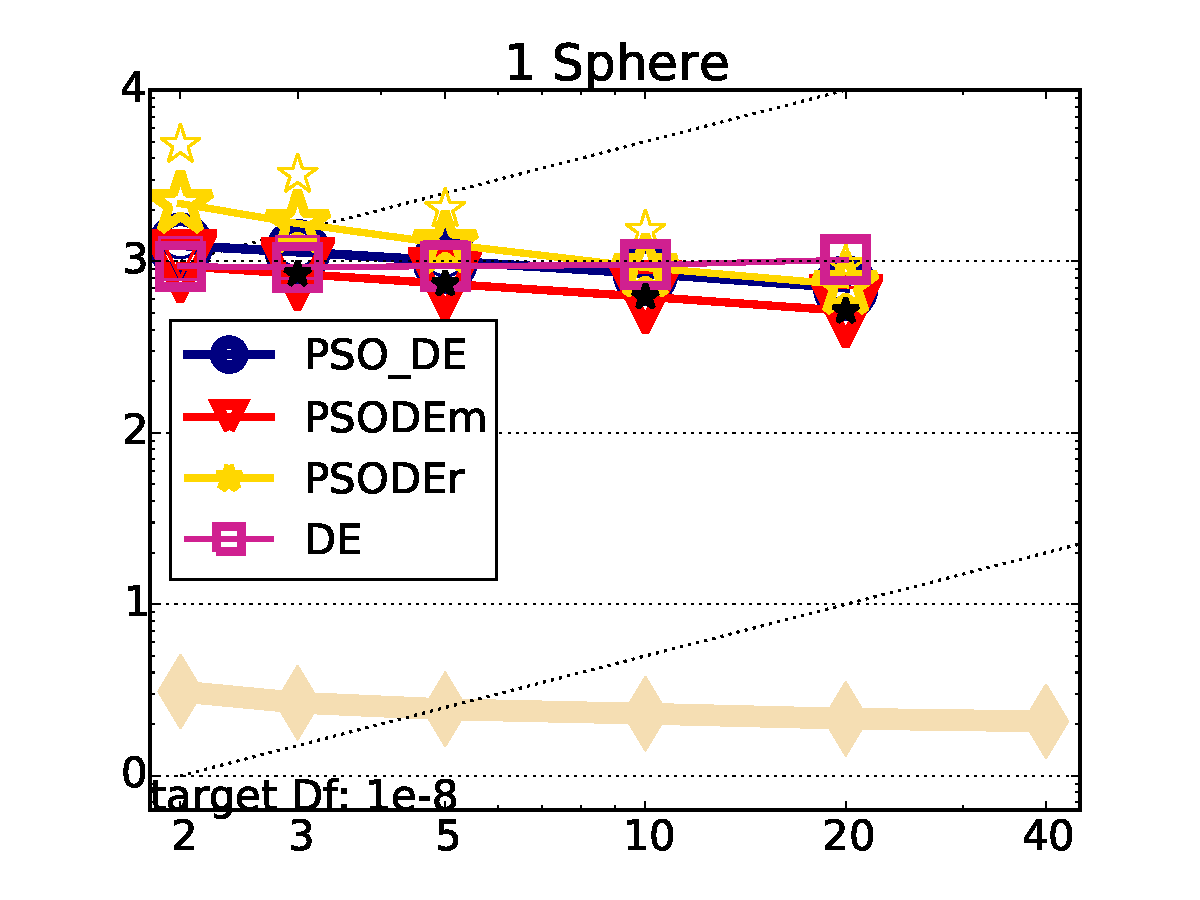
\includegraphics[width=0.25\textwidth, trim=20mm 7mm 15mm 3mm, clip]{ppfigs_f001}&
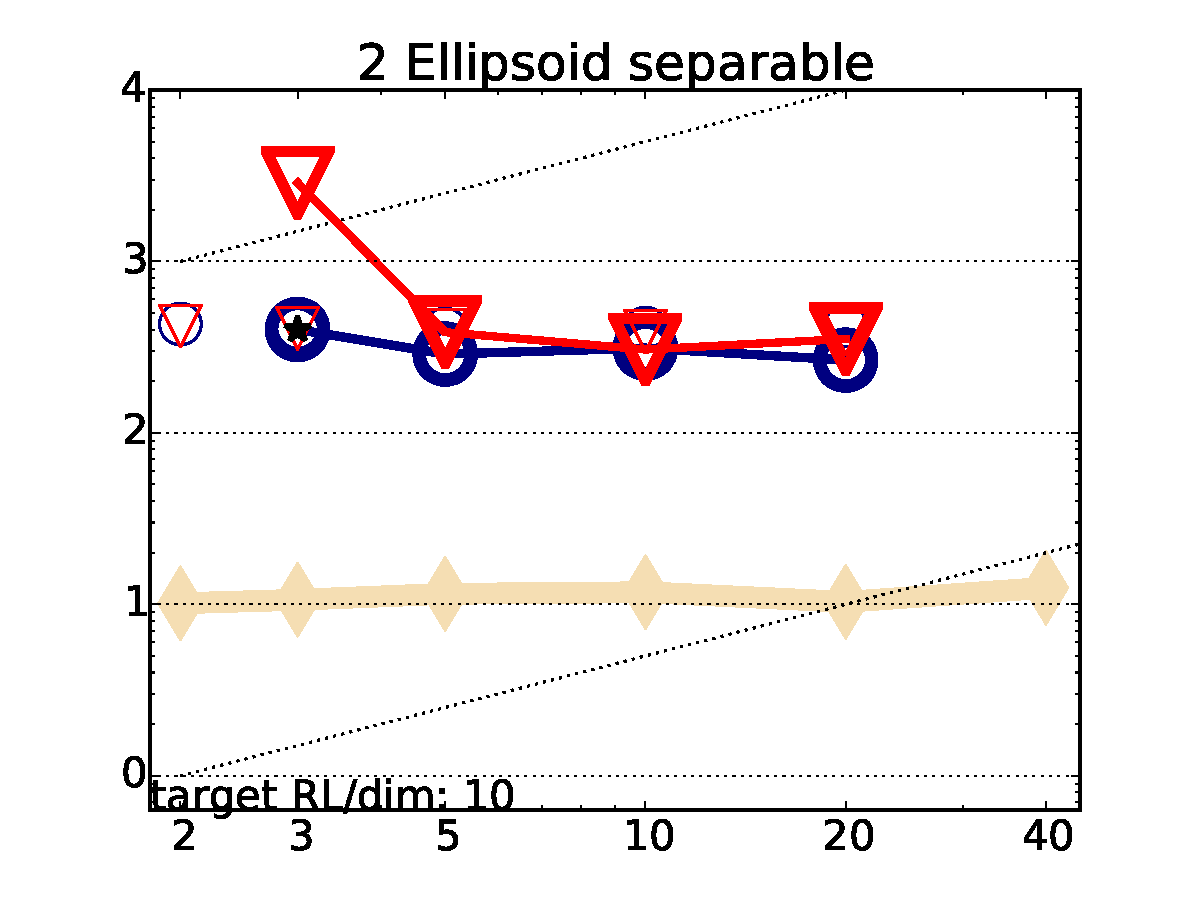
\includegraphics[width=0.25\textwidth, trim=20mm 7mm 15mm 3mm, clip]{ppfigs_f002}&
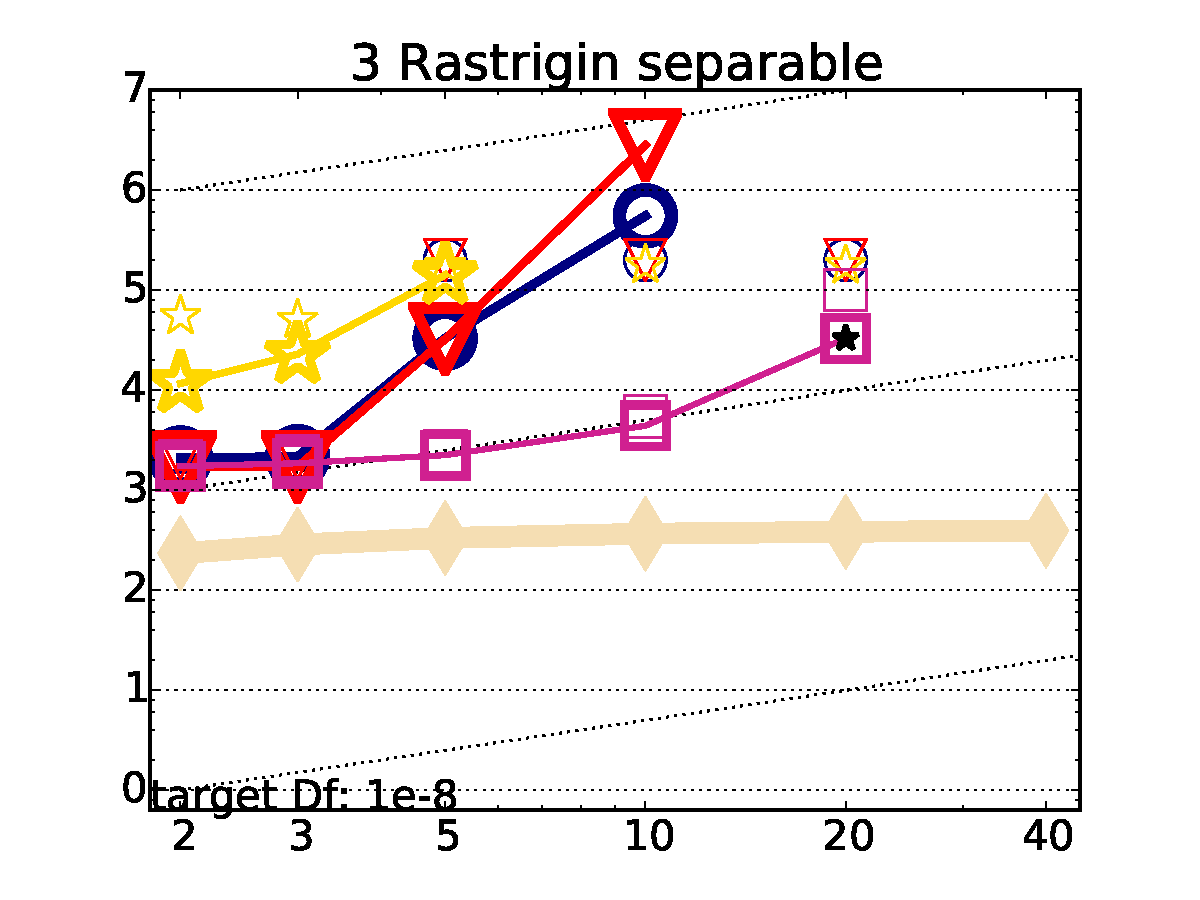
\includegraphics[width=0.25\textwidth, trim=20mm 7mm 15mm 3mm, clip]{ppfigs_f003}&
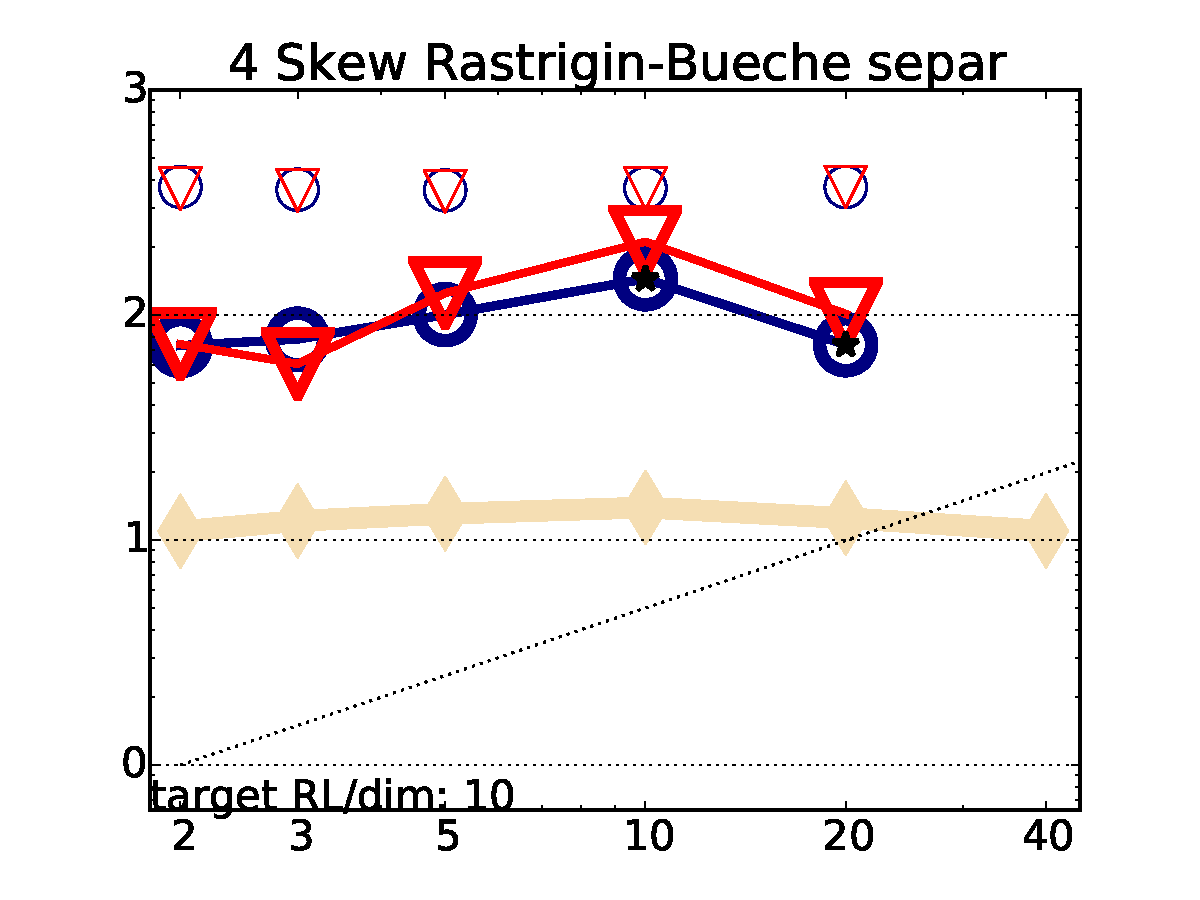
\includegraphics[width=0.25\textwidth, trim=20mm 7mm 15mm 3mm, clip]{ppfigs_f004}\\
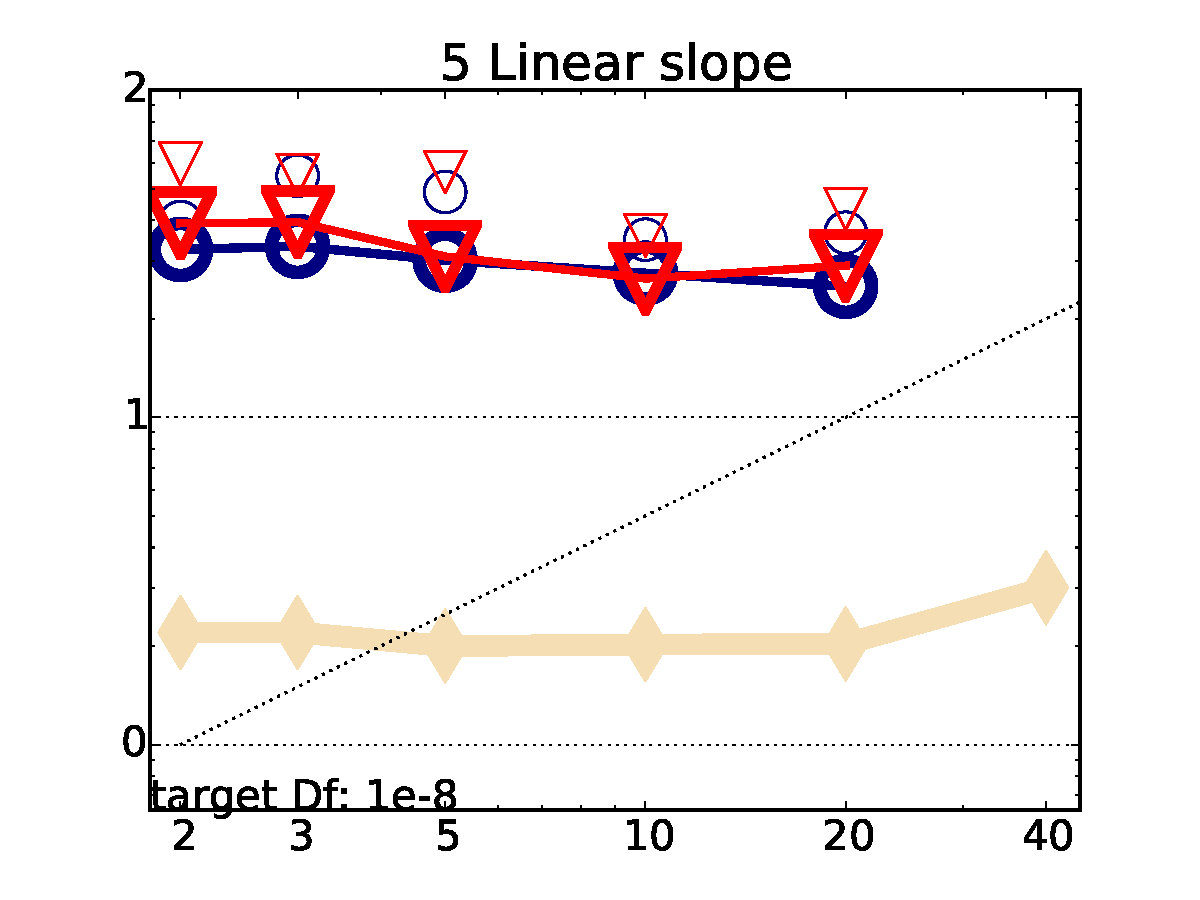
\includegraphics[width=0.25\textwidth, trim=20mm 7mm 15mm 3mm, clip]{ppfigs_f005}&
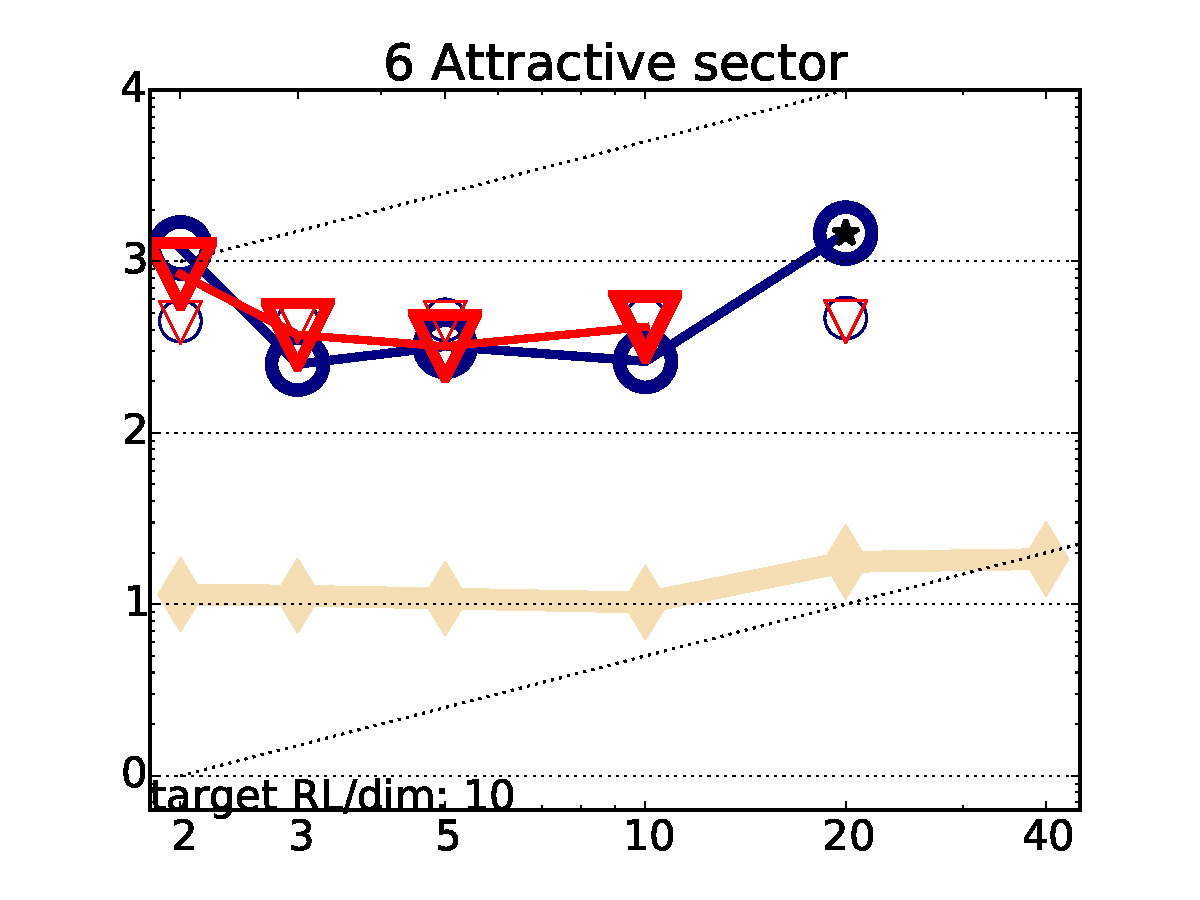
\includegraphics[width=0.25\textwidth, trim=20mm 7mm 15mm 3mm, clip]{ppfigs_f006}&
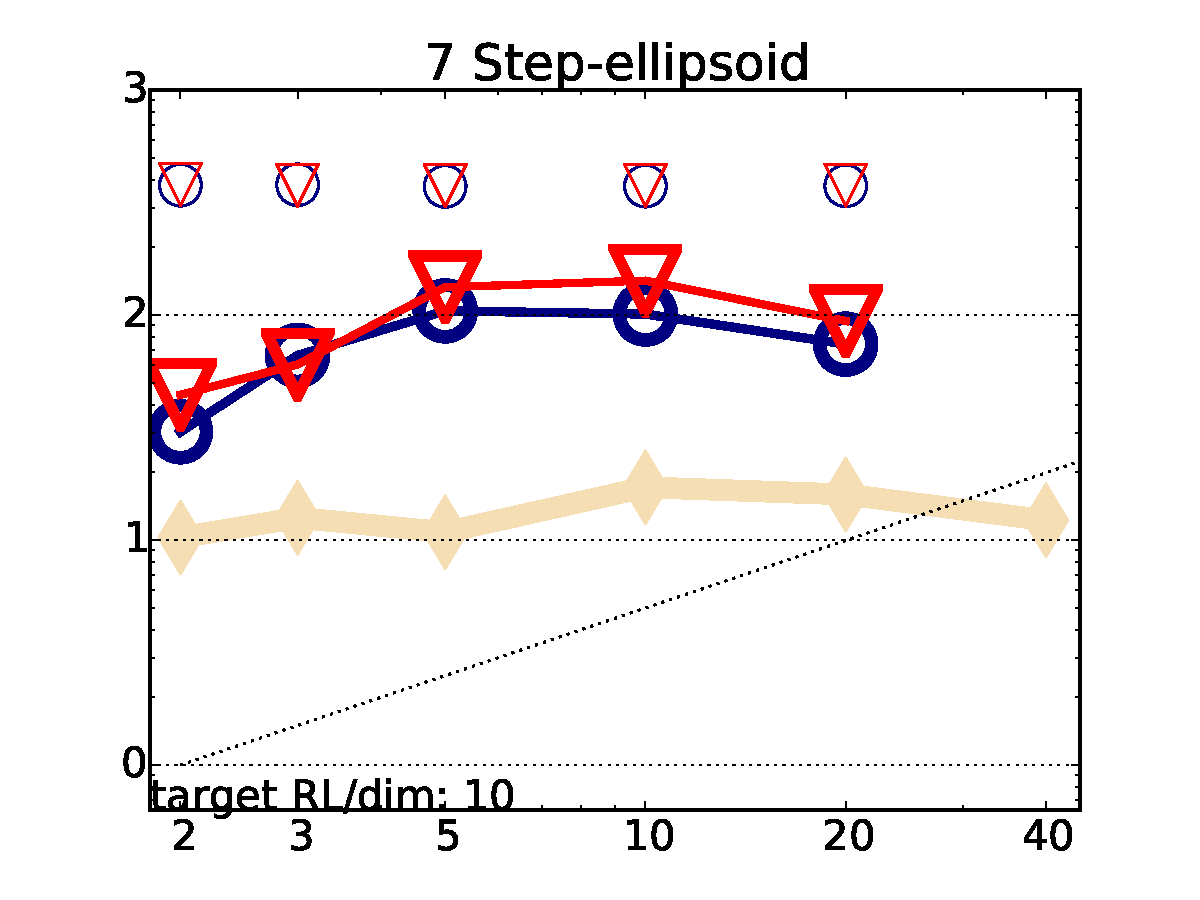
\includegraphics[width=0.25\textwidth, trim=20mm 7mm 15mm 3mm, clip]{ppfigs_f007}&
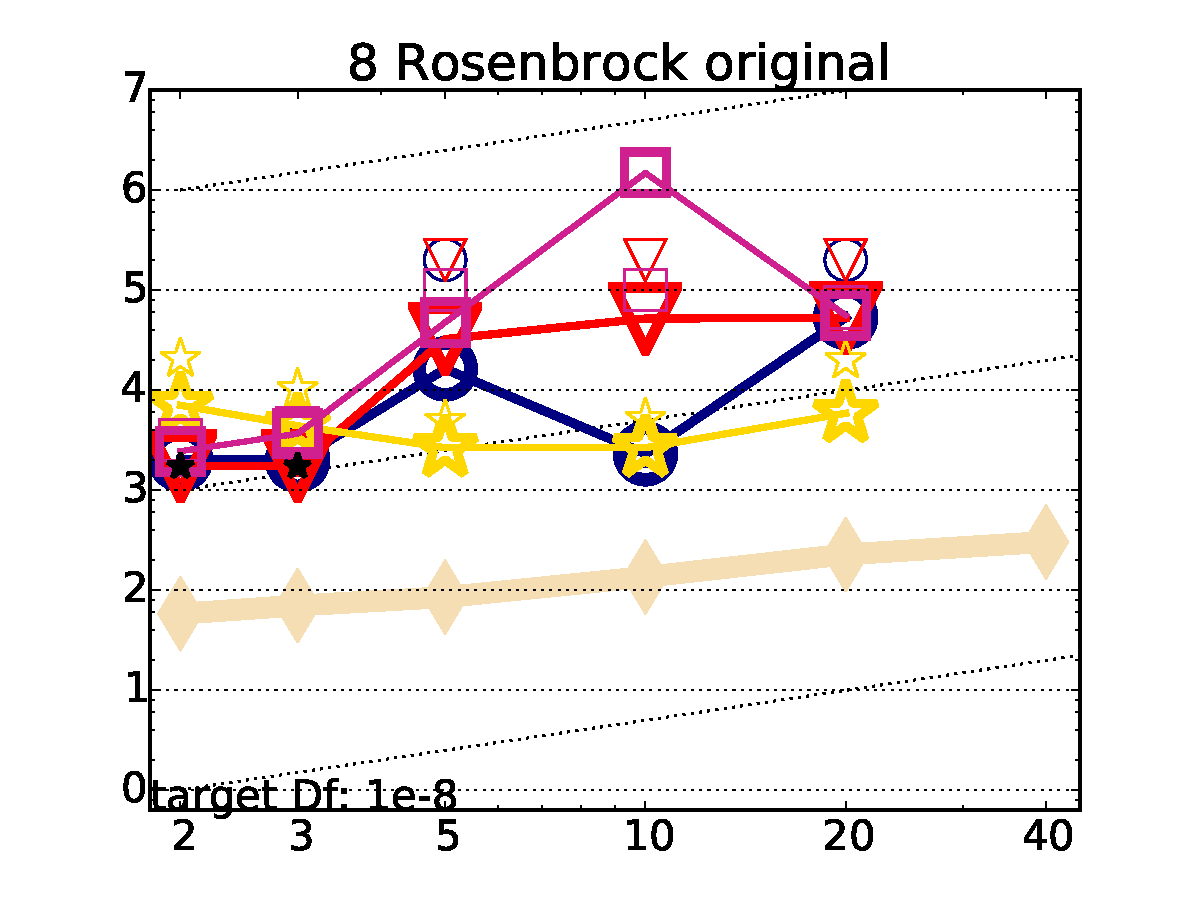
\includegraphics[width=0.25\textwidth, trim=20mm 7mm 15mm 3mm, clip]{ppfigs_f008}\\
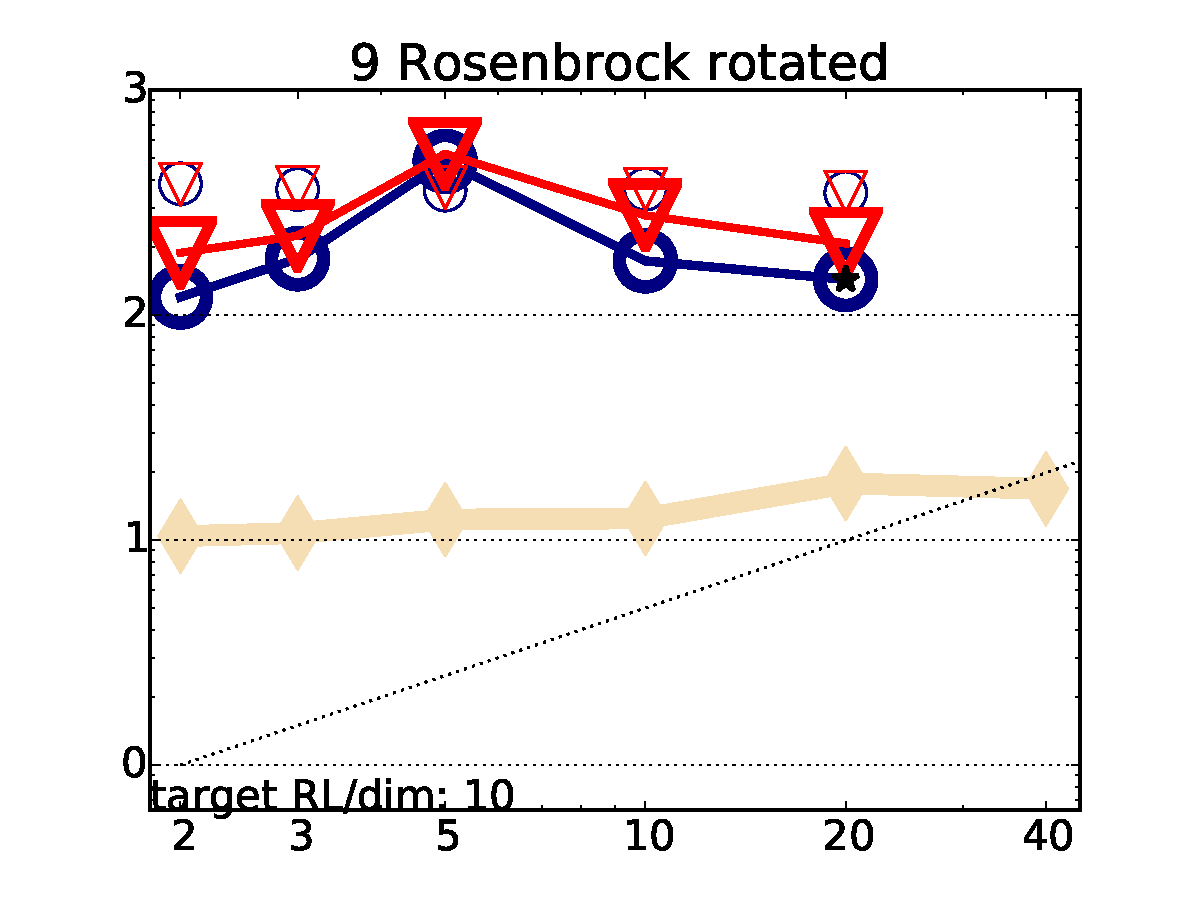
\includegraphics[width=0.25\textwidth, trim=20mm 7mm 15mm 3mm, clip]{ppfigs_f009}&
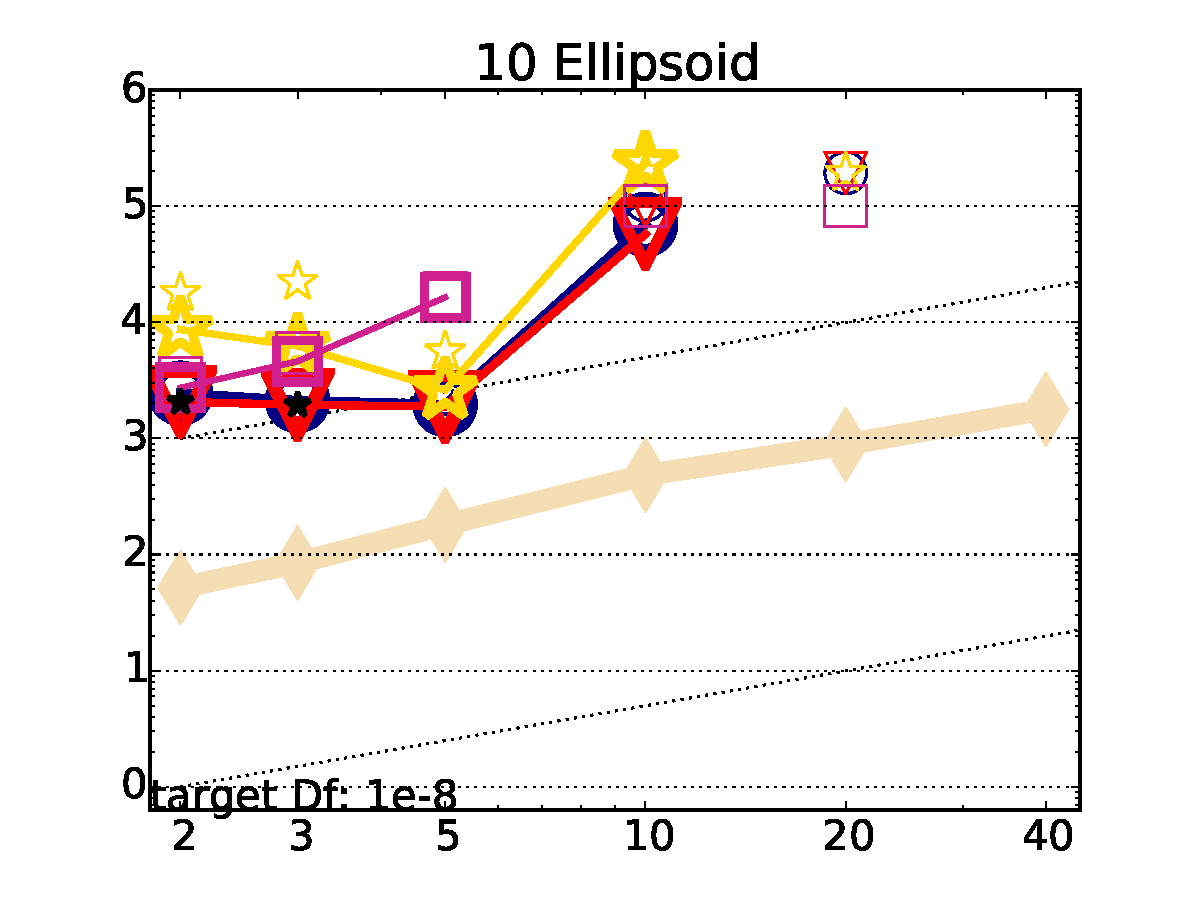
\includegraphics[width=0.25\textwidth, trim=20mm 7mm 15mm 3mm, clip]{ppfigs_f010}&
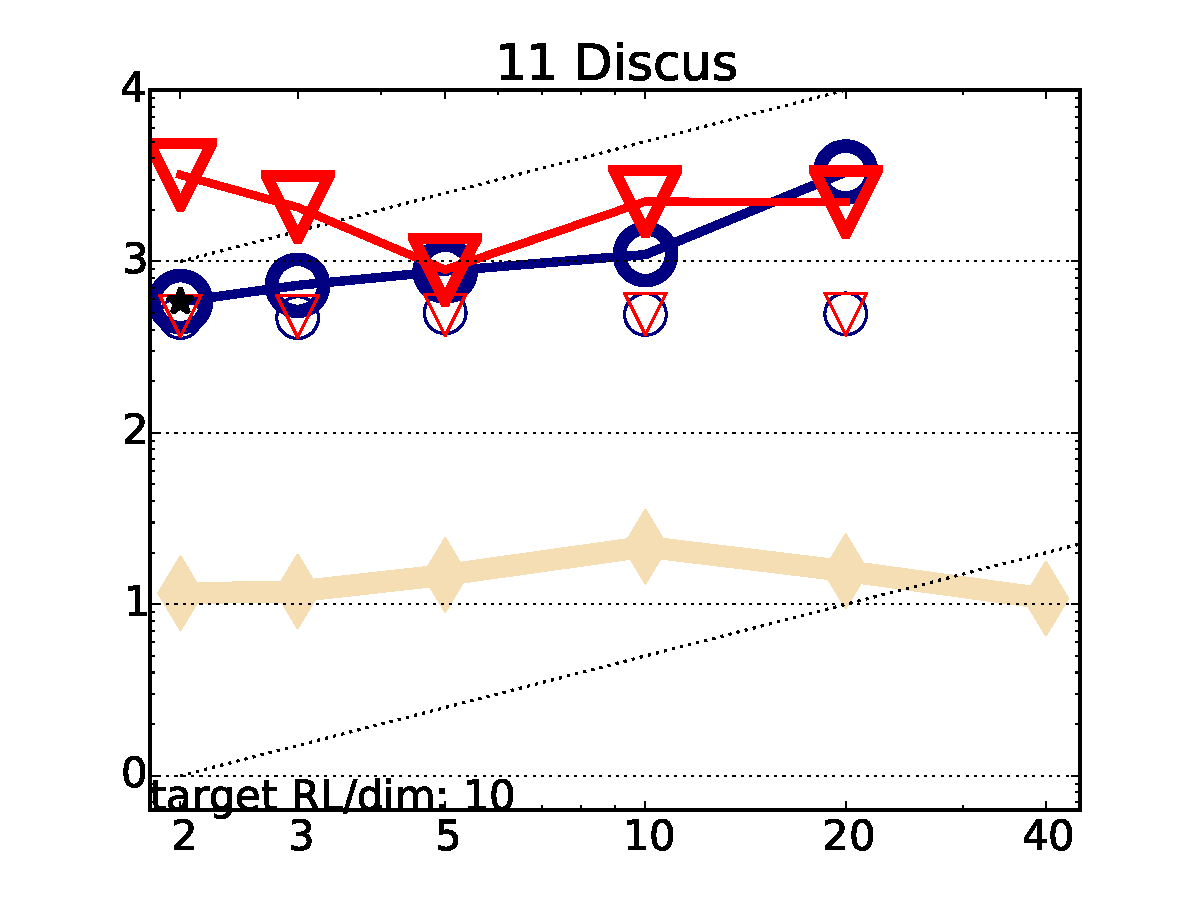
\includegraphics[width=0.25\textwidth, trim=20mm 7mm 15mm 3mm, clip]{ppfigs_f011}&
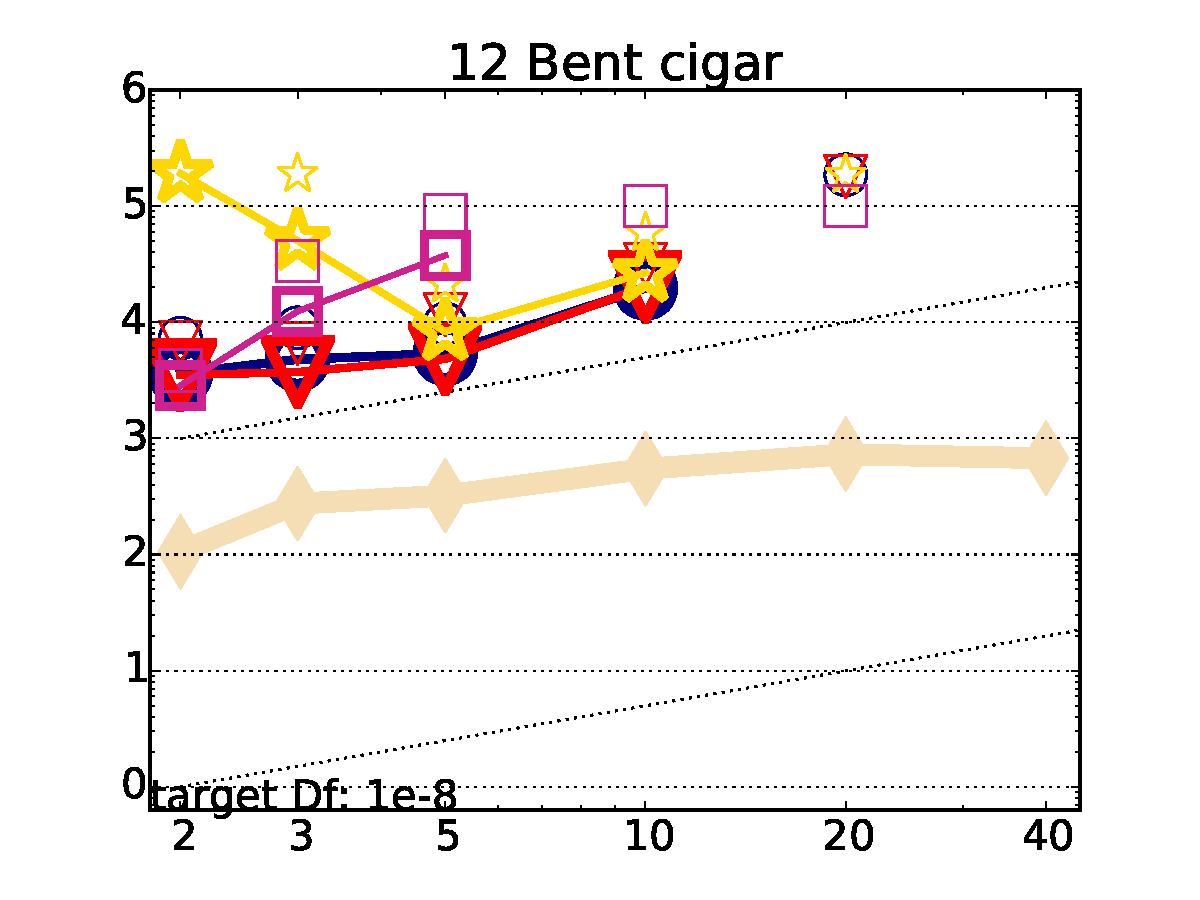
\includegraphics[width=0.25\textwidth, trim=20mm 7mm 15mm 3mm, clip]{ppfigs_f012}\\
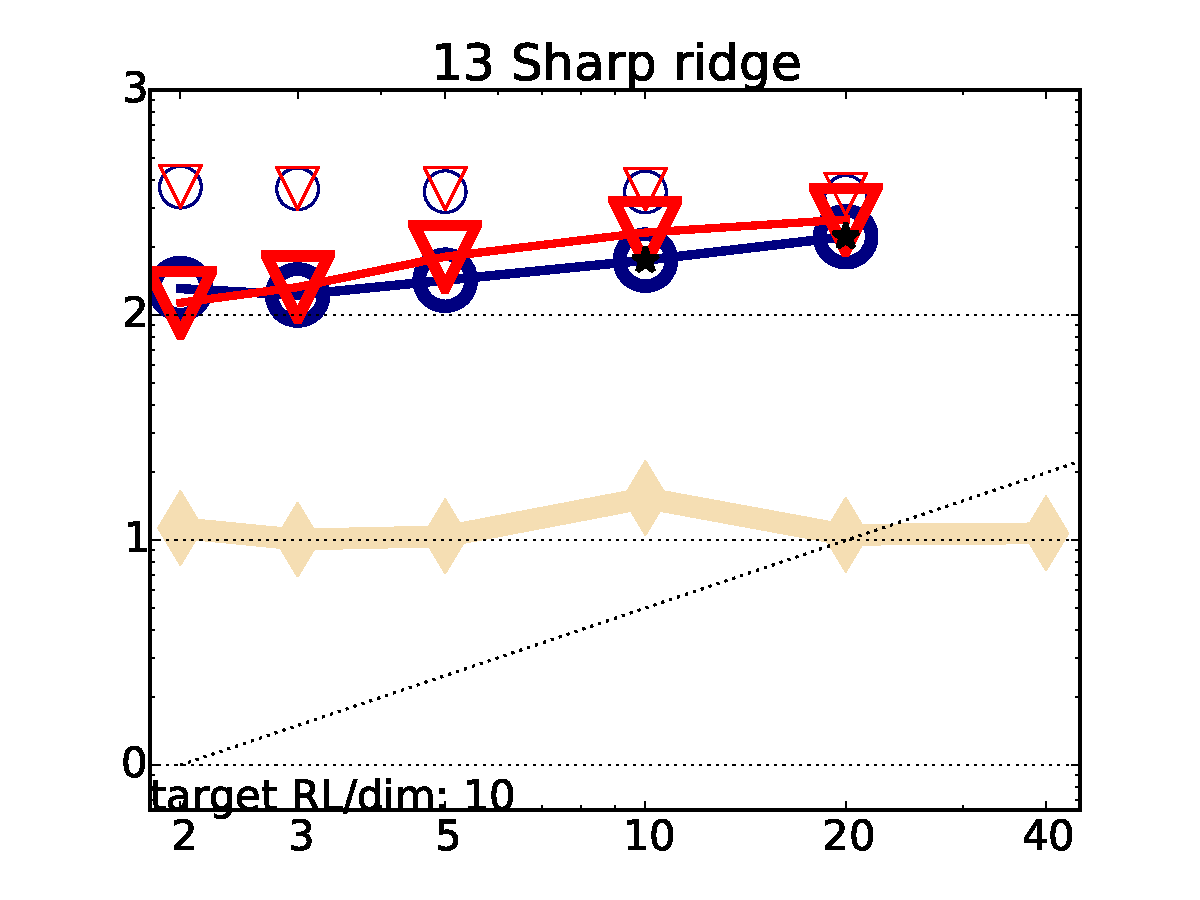
\includegraphics[width=0.25\textwidth, trim=20mm 7mm 15mm 3mm, clip]{ppfigs_f013}&
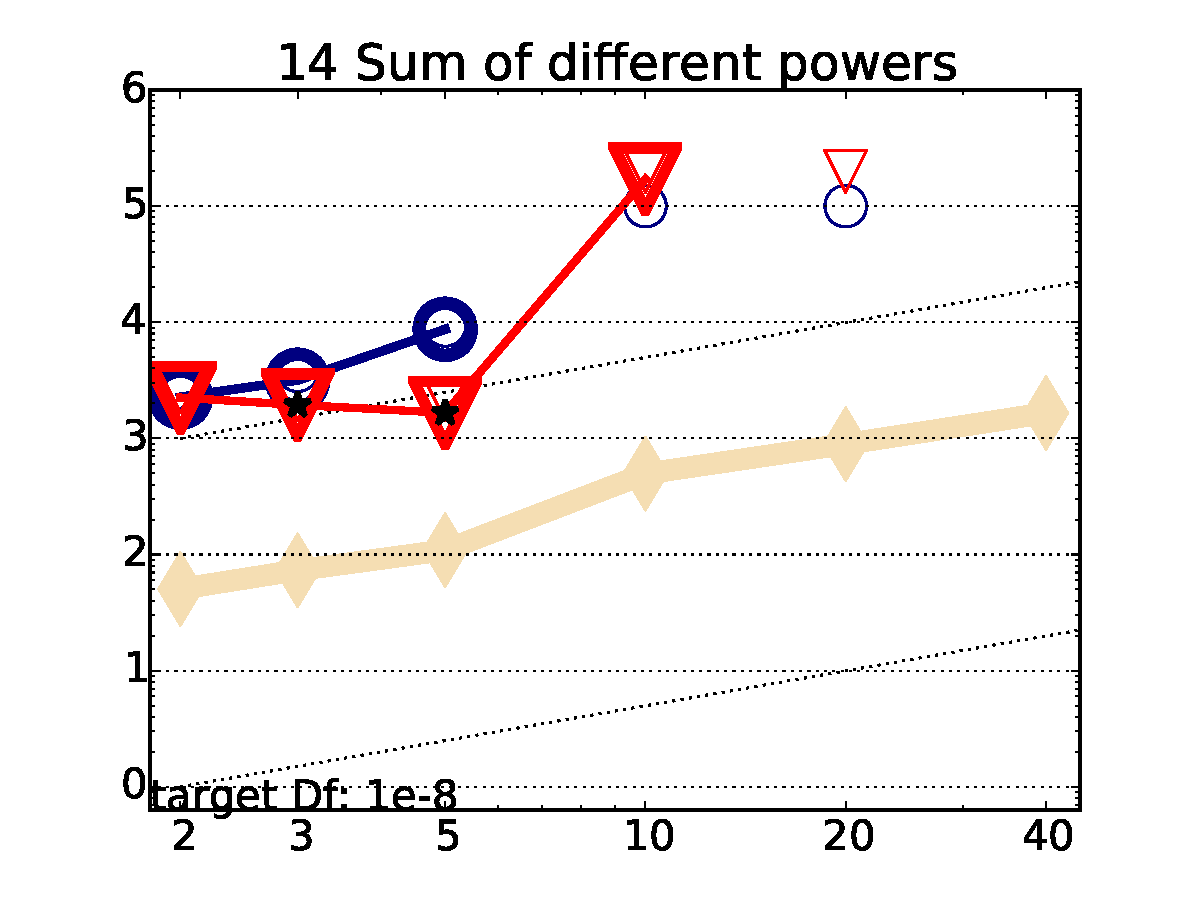
\includegraphics[width=0.25\textwidth, trim=20mm 7mm 15mm 3mm, clip]{ppfigs_f014}&
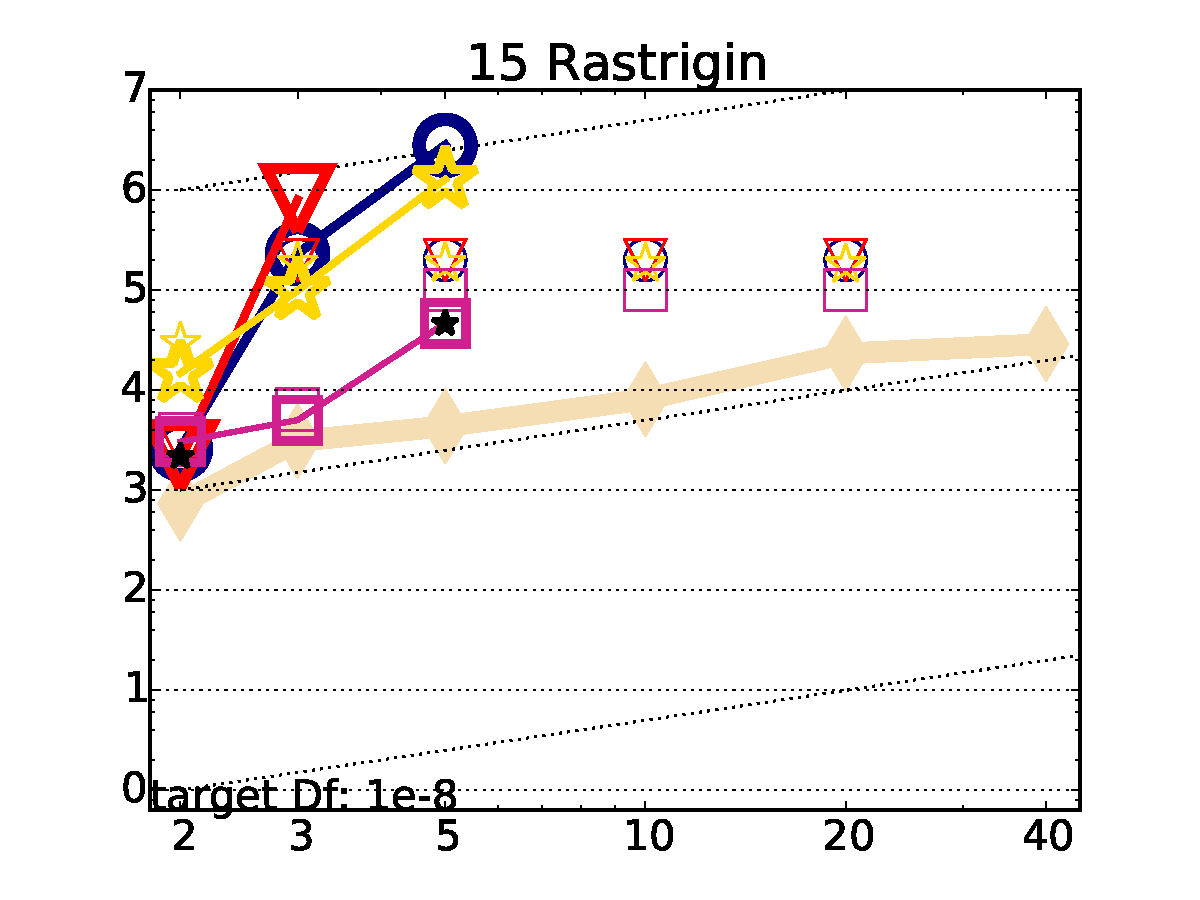
\includegraphics[width=0.25\textwidth, trim=20mm 7mm 15mm 3mm, clip]{ppfigs_f015}&
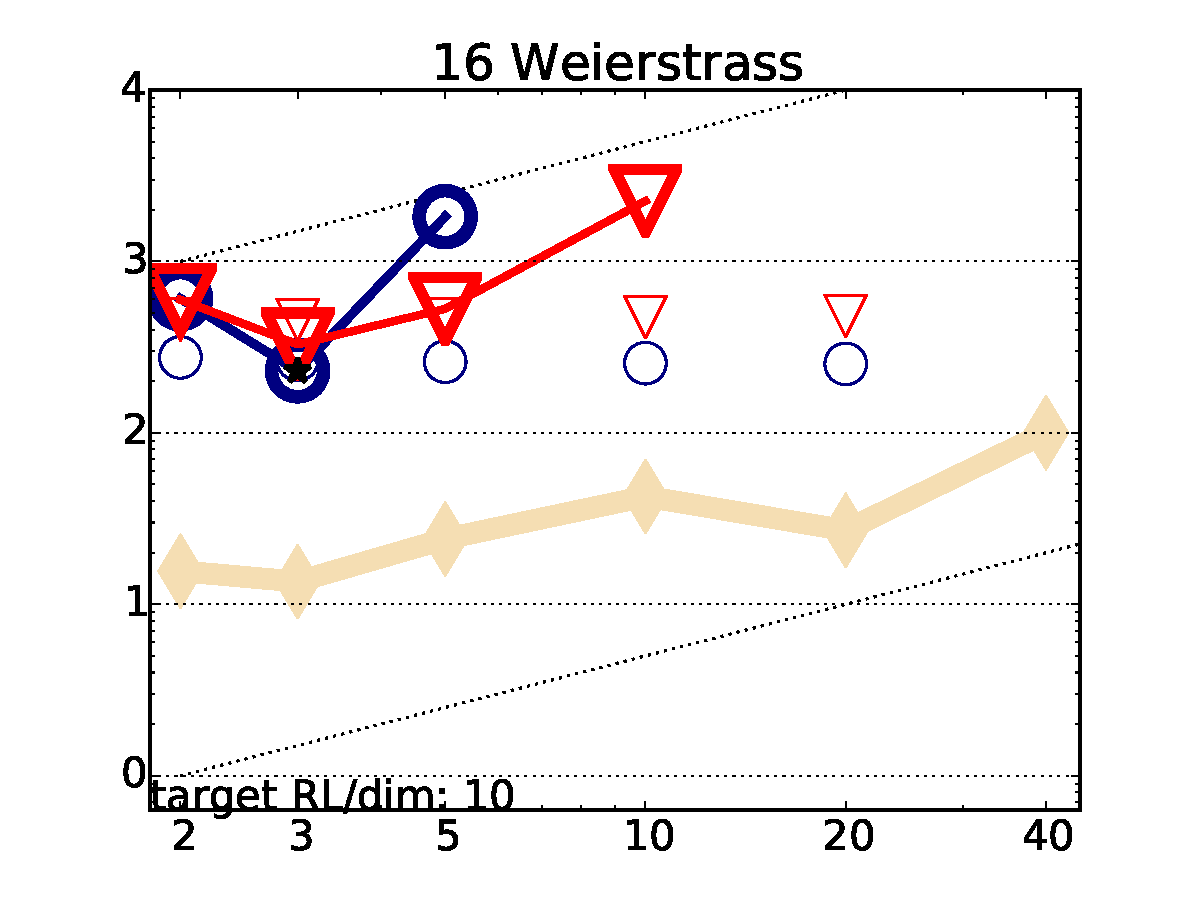
\includegraphics[width=0.25\textwidth, trim=20mm 7mm 15mm 3mm, clip]{ppfigs_f016}\\
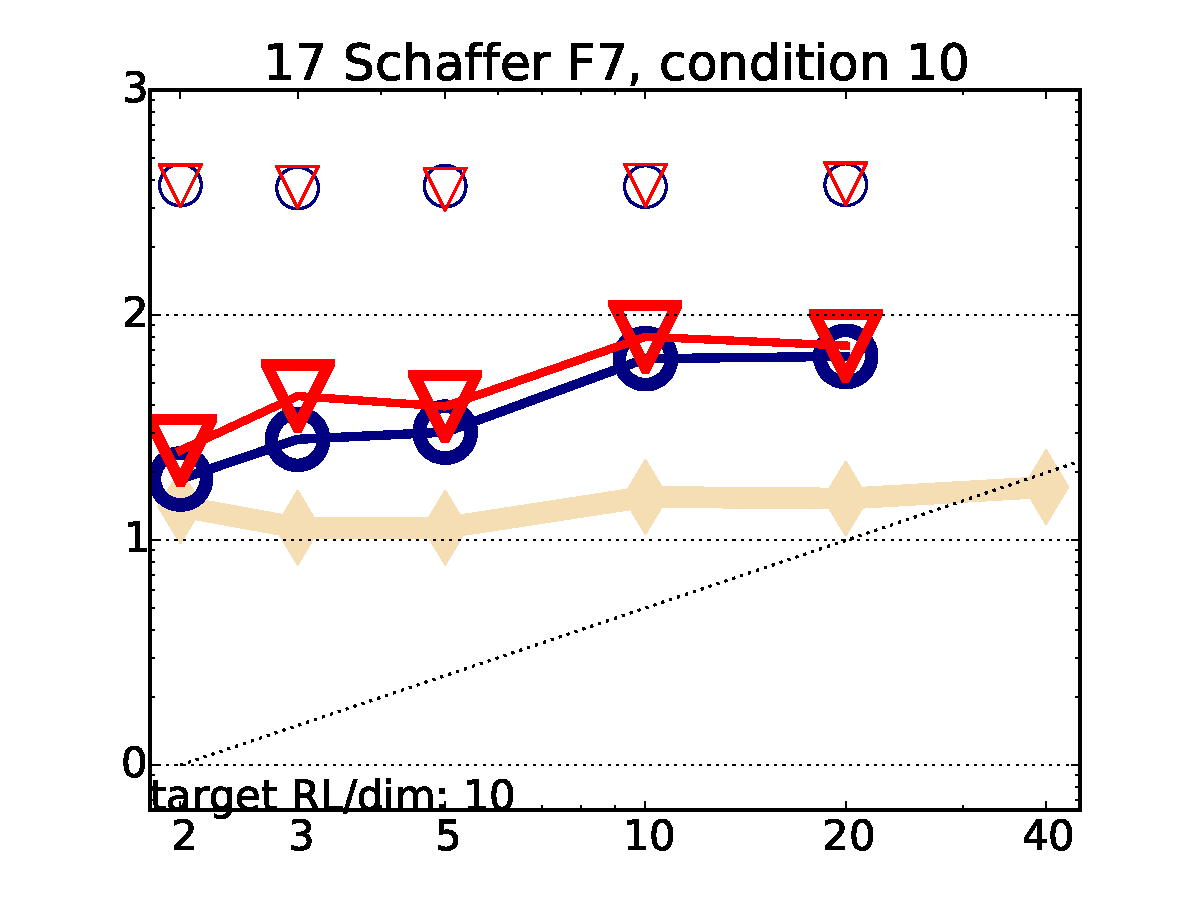
\includegraphics[width=0.25\textwidth, trim=20mm 7mm 15mm 3mm, clip]{ppfigs_f017}&
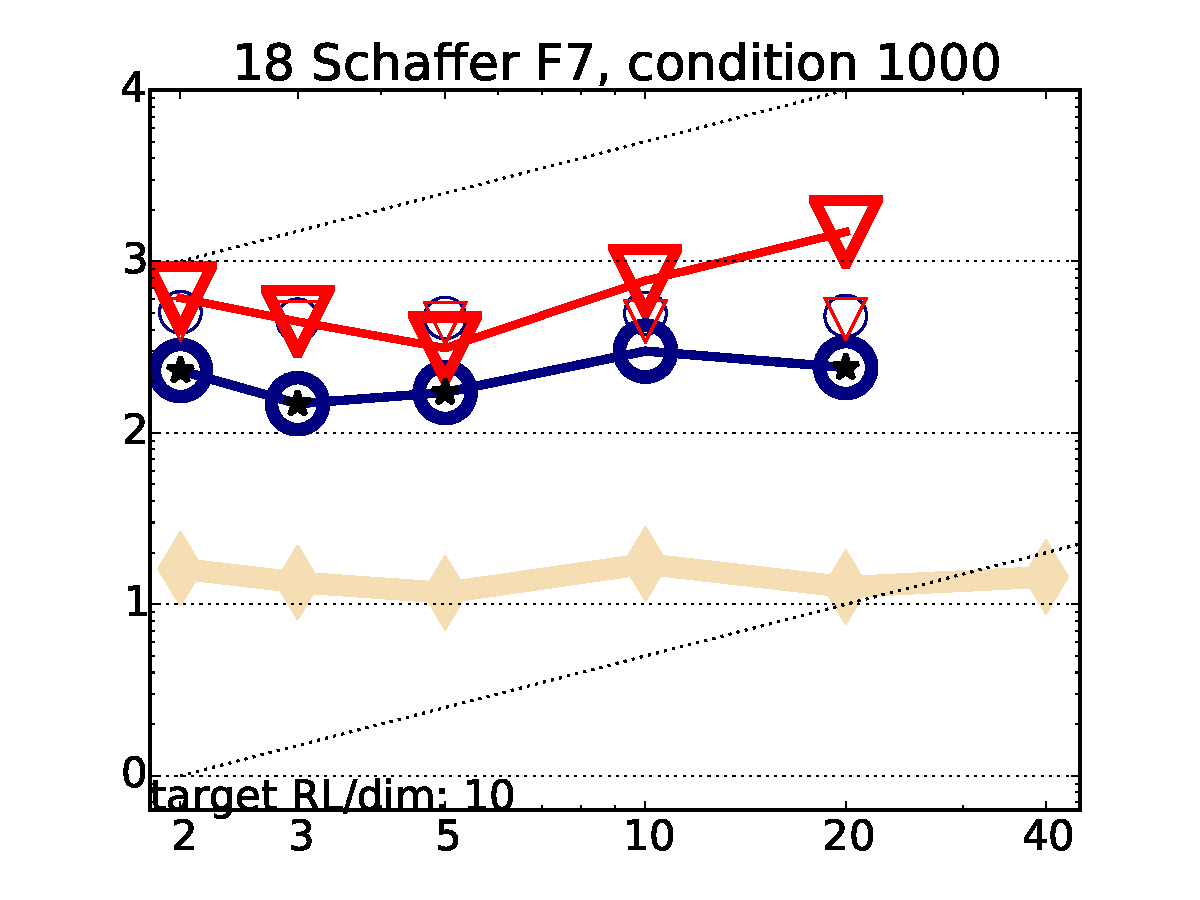
\includegraphics[width=0.25\textwidth, trim=20mm 7mm 15mm 3mm, clip]{ppfigs_f018}&
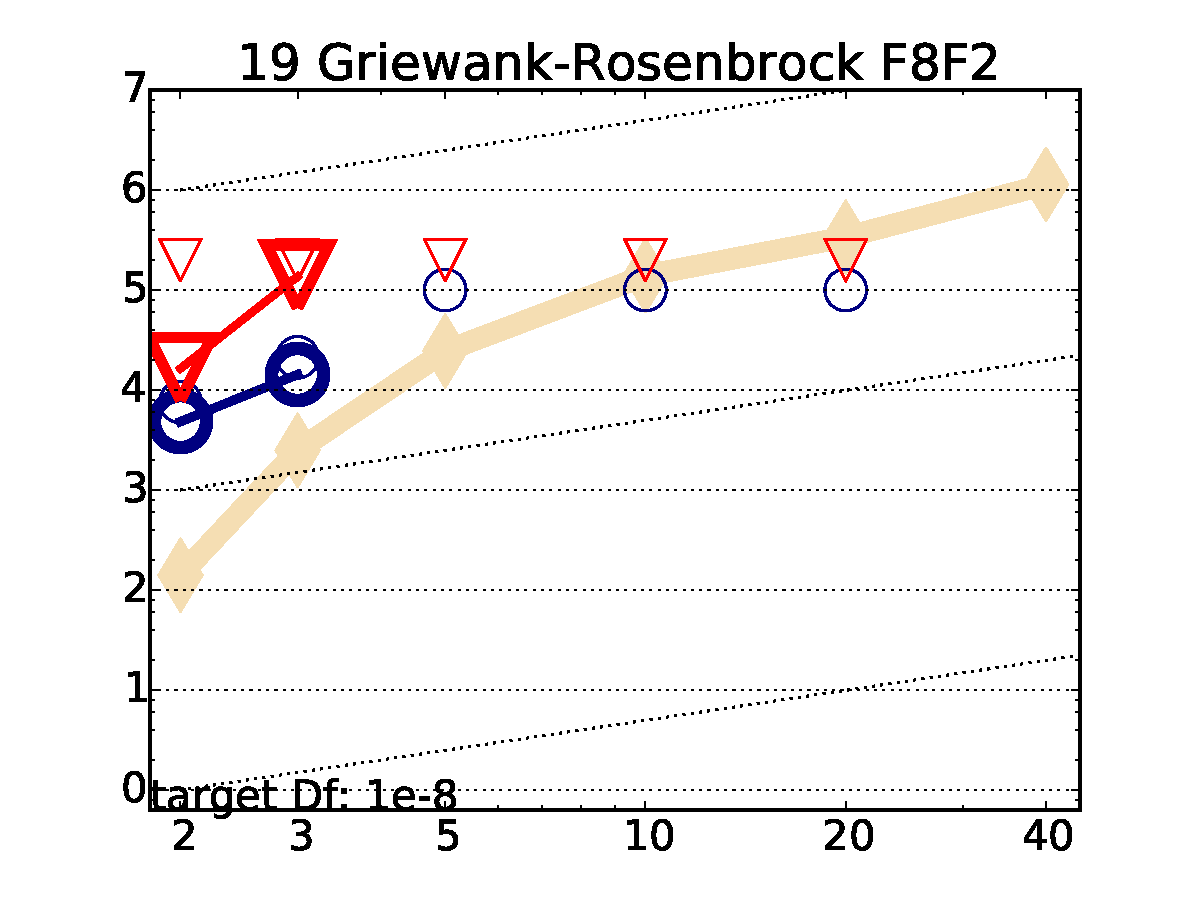
\includegraphics[width=0.25\textwidth, trim=20mm 7mm 15mm 3mm, clip]{ppfigs_f019}&
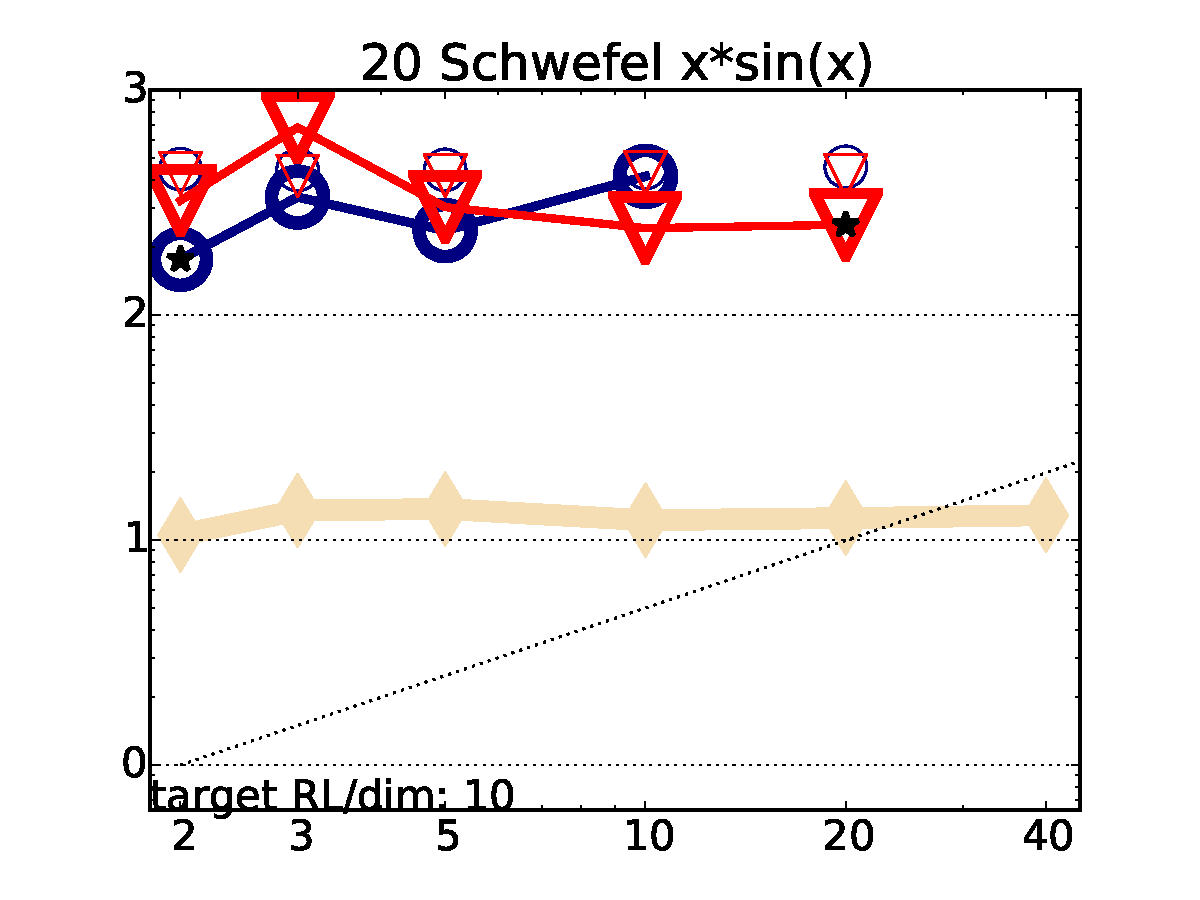
\includegraphics[width=0.25\textwidth, trim=20mm 7mm 15mm 3mm, clip]{ppfigs_f020}\\
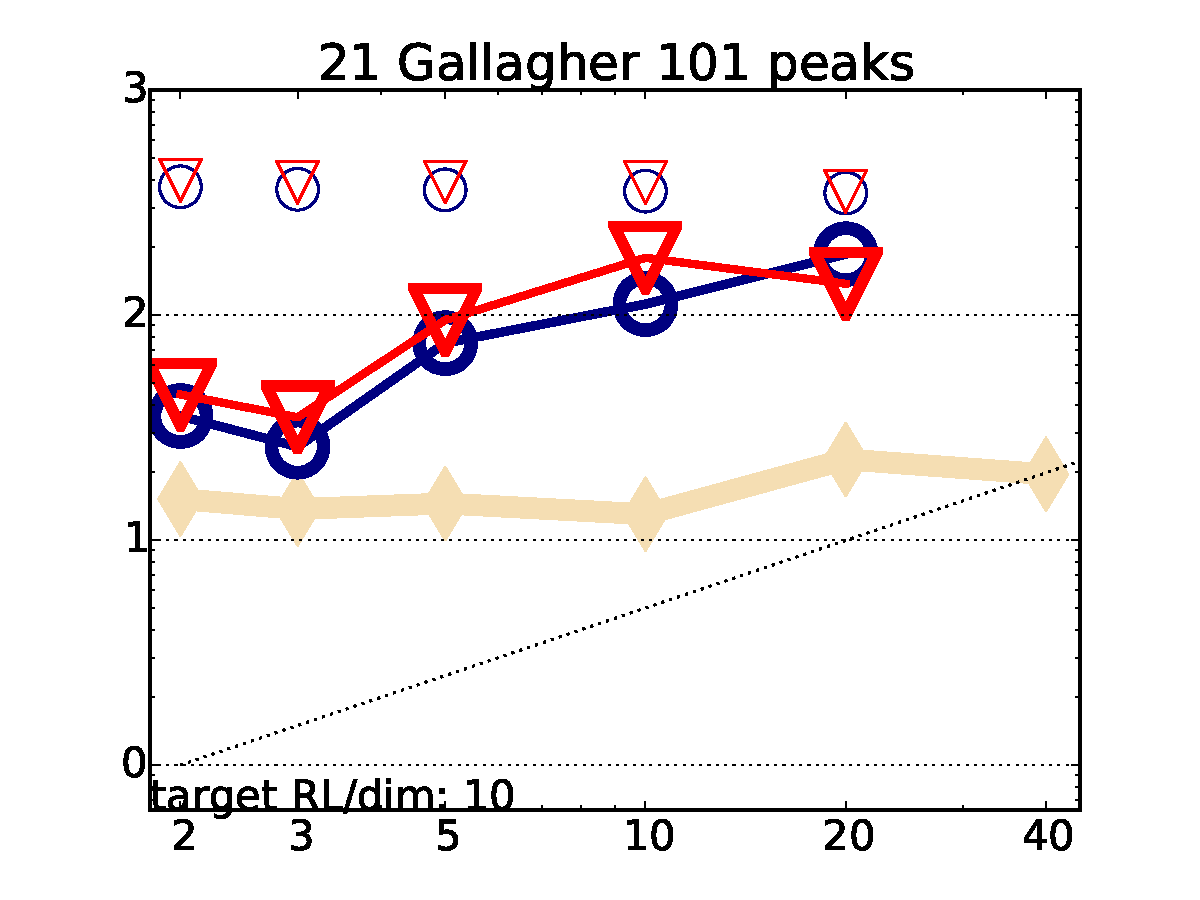
\includegraphics[width=0.25\textwidth, trim=20mm 7mm 15mm 3mm, clip]{ppfigs_f021}&
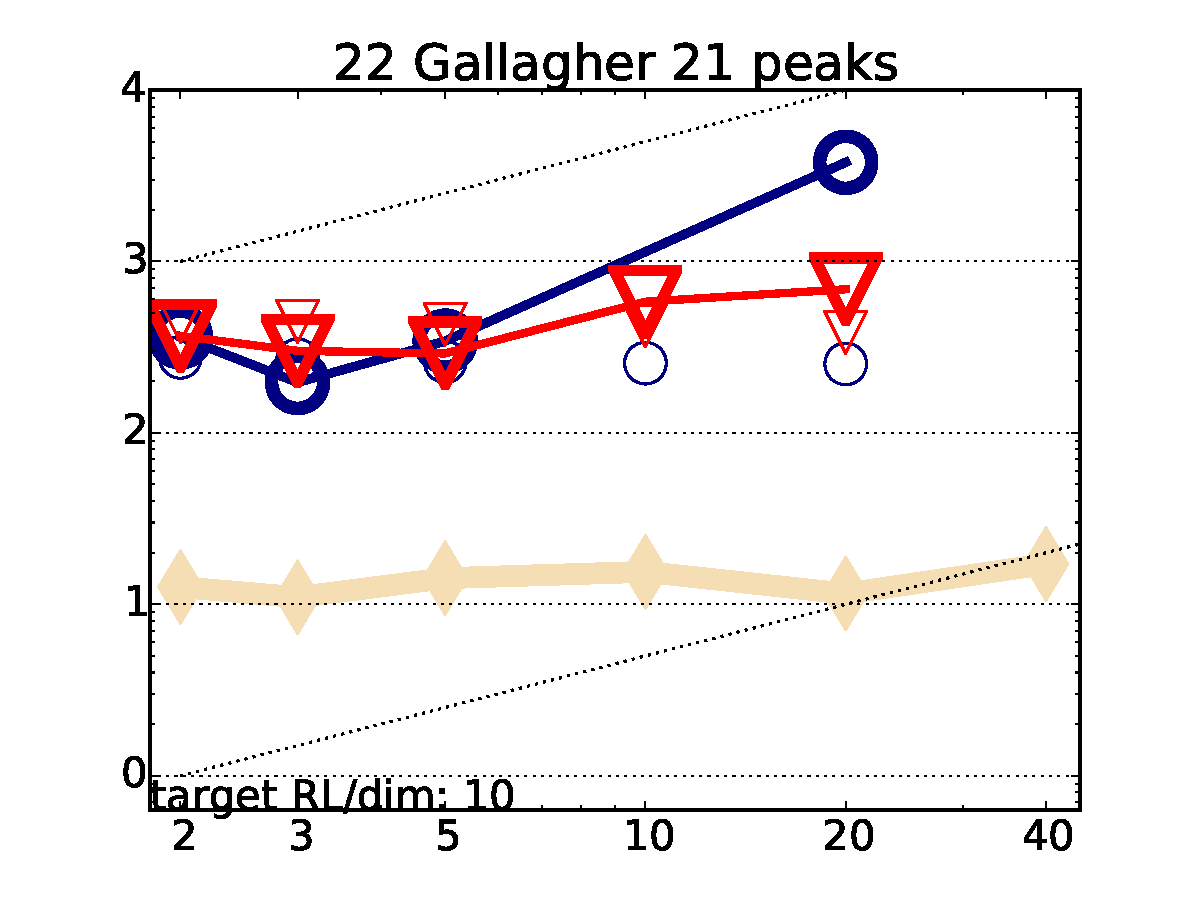
\includegraphics[width=0.25\textwidth, trim=20mm 7mm 15mm 3mm, clip]{ppfigs_f022}&
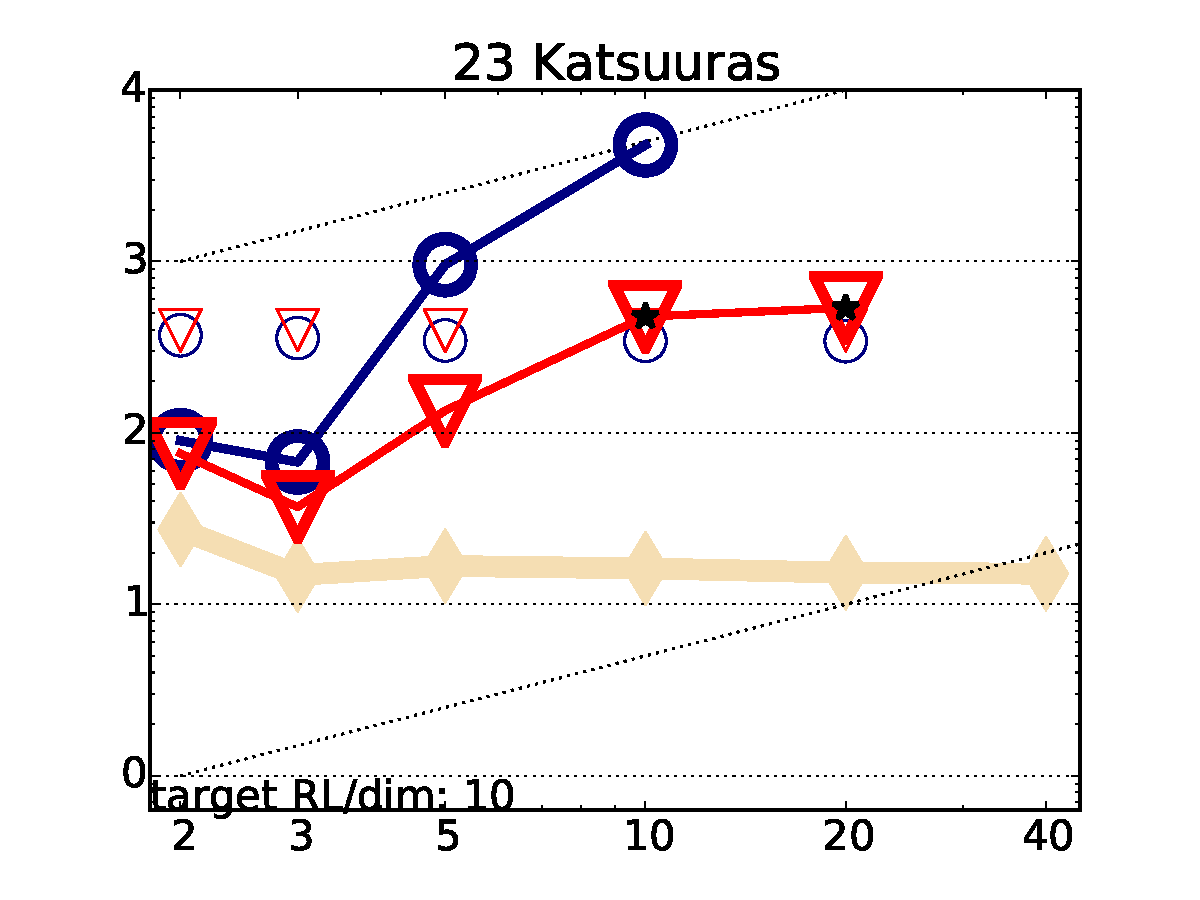
\includegraphics[width=0.25\textwidth, trim=20mm 7mm 15mm 3mm, clip]{ppfigs_f023}&
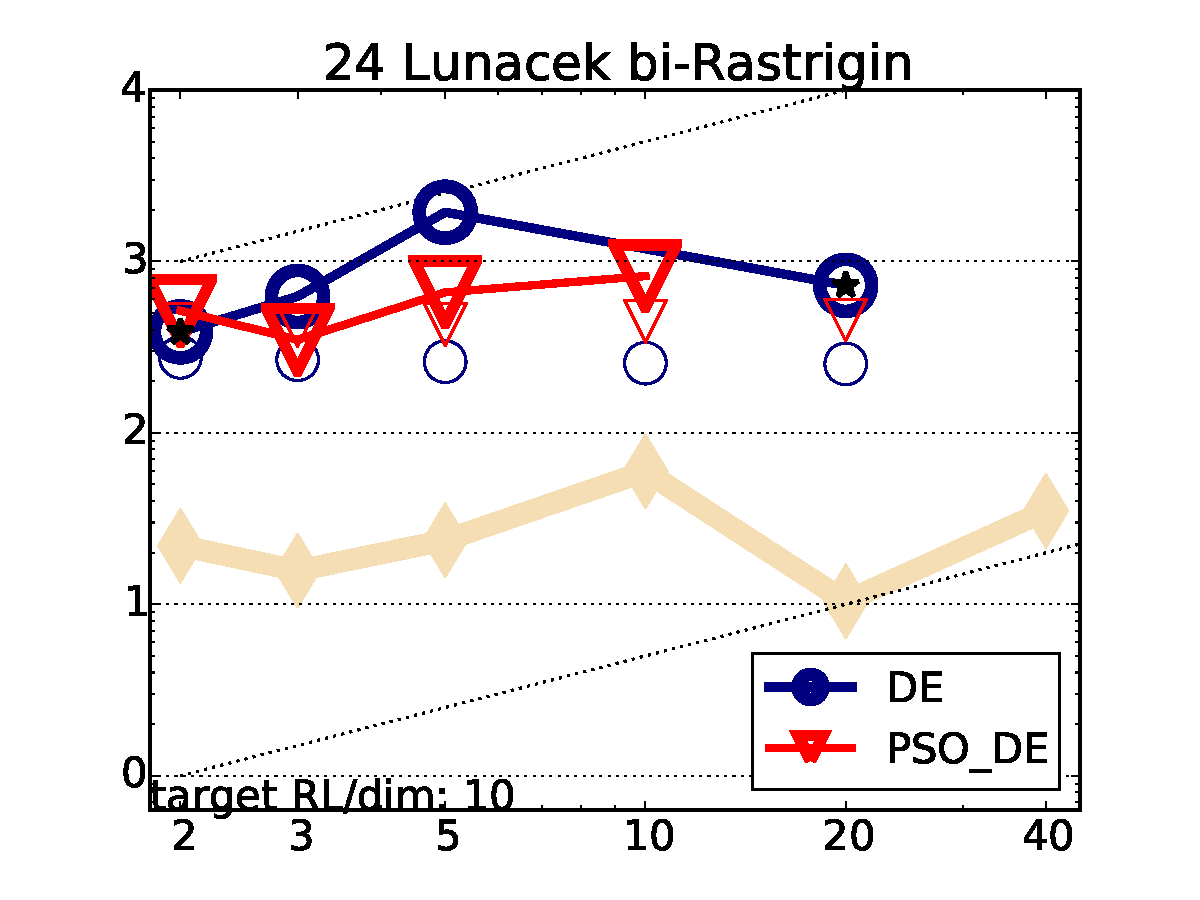
\includegraphics[width=0.25\textwidth, trim=20mm 7mm 15mm 3mm, clip]{ppfigs_f024}
\end{tabular}
\vspace*{-0.2cm}
\caption[Expected running time divided by dimension versus dimension]{
\label{fig:scaling}
% command defined in bbob_pproc_commands.tex:
\bbobppfigslegend{$f_1$ and $f_{24}$}.  % \algorithmA can be defined above, see above
% \input{\bbobdatapath ppfigs}
}
% The legend is in file \bbobdatapath ppfigs.tex
% While compiling this document, if the following error comes up:
% ! Undefined control sequence.
% try uncommenting line 9 and 10
\end{figure}
%%%%%%%%%%%%%%%%%%%%%%%%%%%%%%%%%%%%%%%%%%%%%%%%%%%%%%%%%%%%%%%%%%%%%%%%%%%%%%%
%%%%%%%%%%%%%%%%%%%%%%%%%%%%%%%%%%%%%%%%%%%%%%%%%%%%%%%%%%%%%%%%%%%%%%%%%%%%%%%
\begin{figure}
\begin{tabular}{*{4}{@{}c@{}}}
    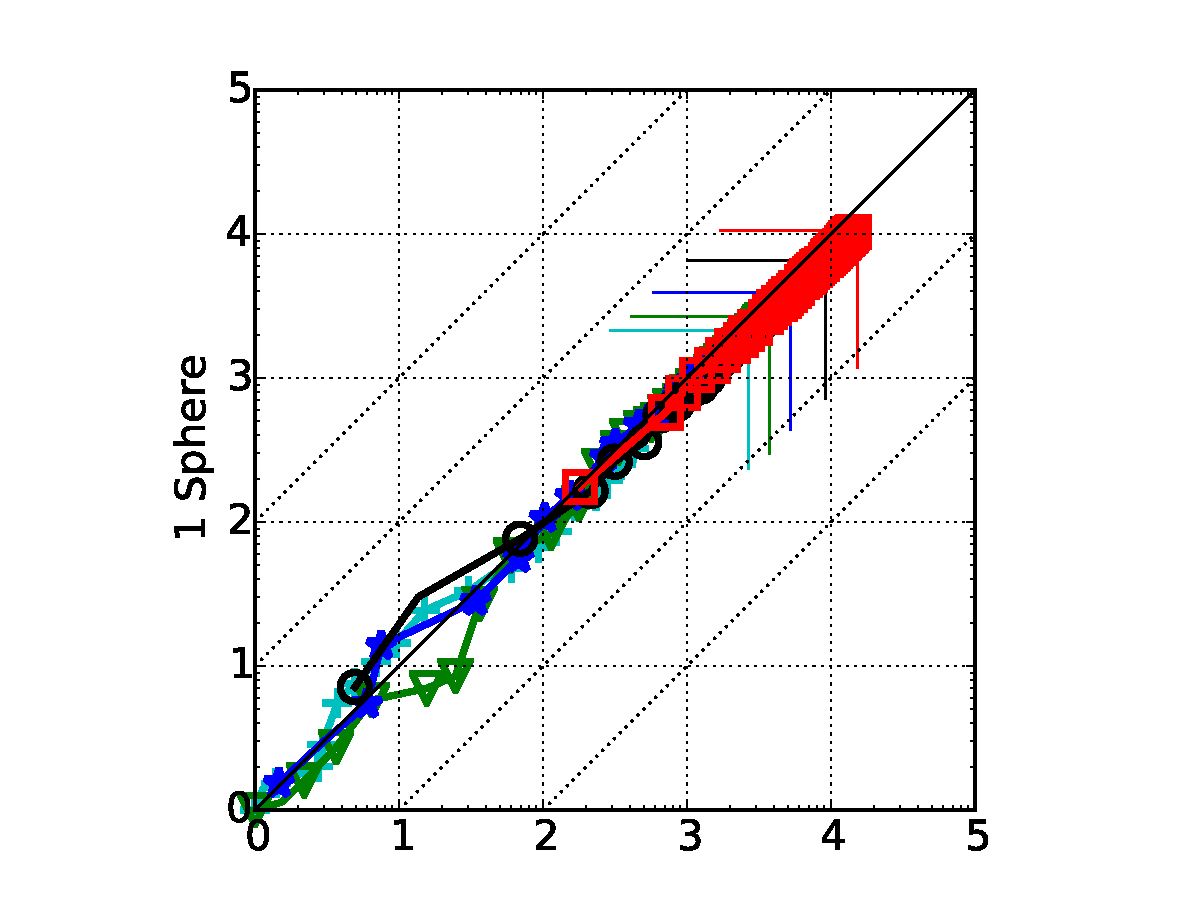
\includegraphics[width=0.25\textwidth, trim= 29mm 8.5mm 35mm 13mm, clip]{ppscatter_f001}&
    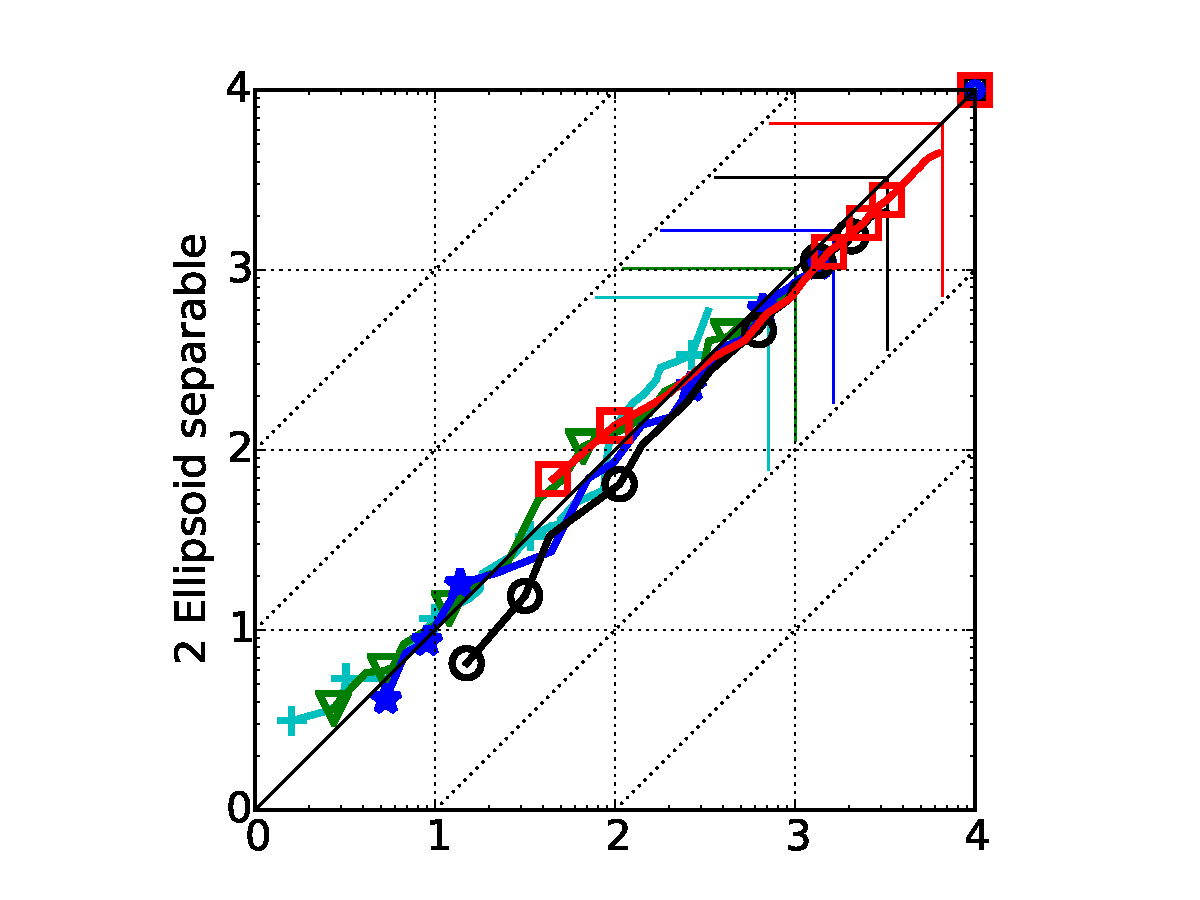
\includegraphics[width=0.25\textwidth, trim= 29mm 8.5mm 35mm 13mm, clip]{ppscatter_f002}&
    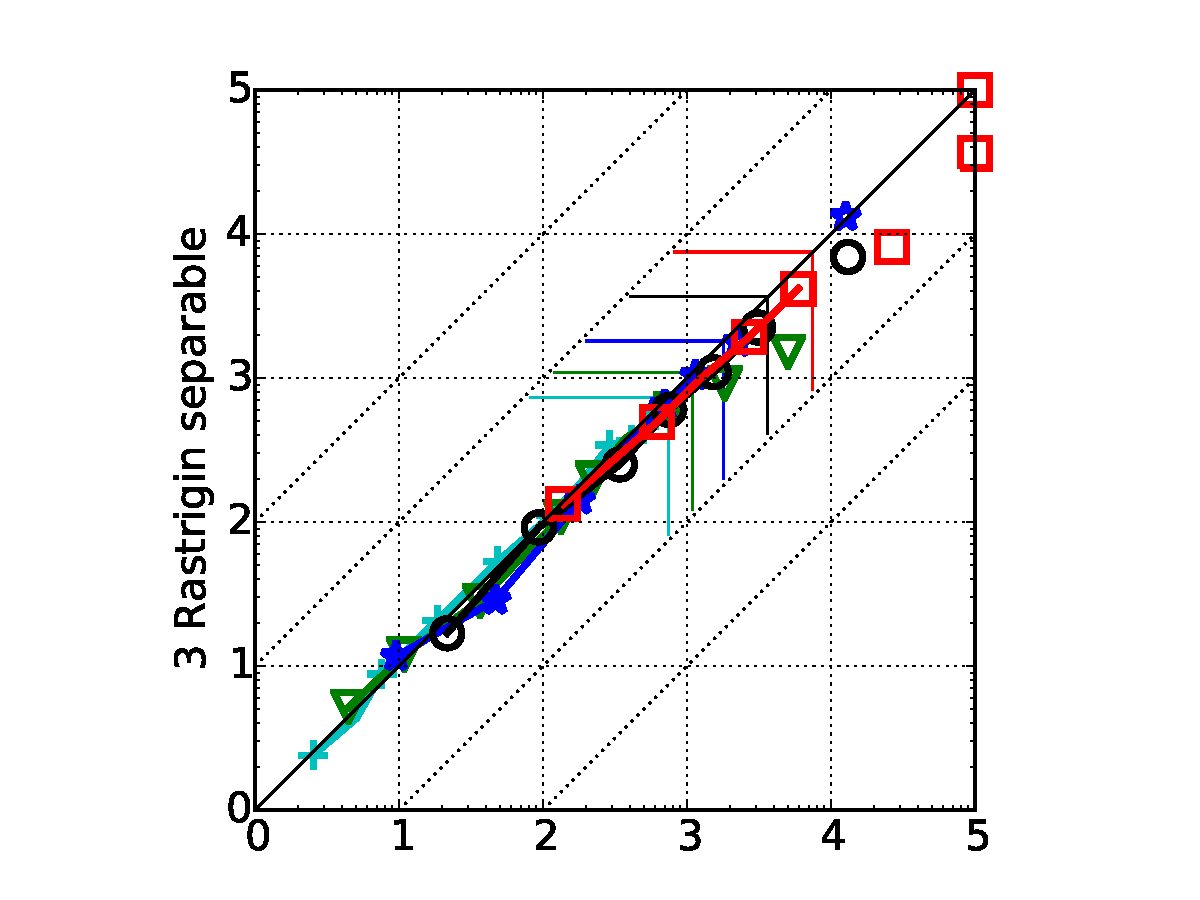
\includegraphics[width=0.25\textwidth, trim= 29mm 8.5mm 35mm 13mm, clip]{ppscatter_f003}&
    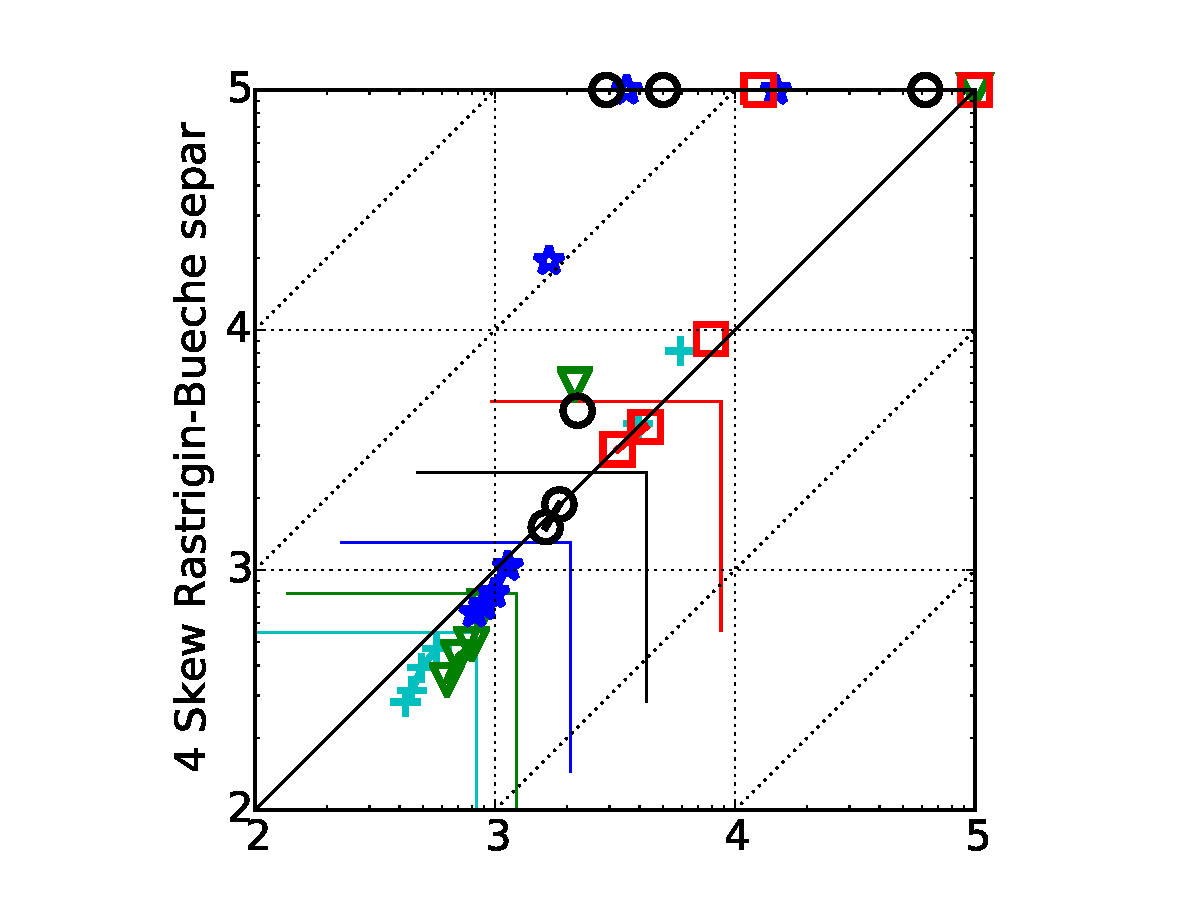
\includegraphics[width=0.25\textwidth, trim= 29mm 8.5mm 35mm 13mm, clip]{ppscatter_f004}\\
    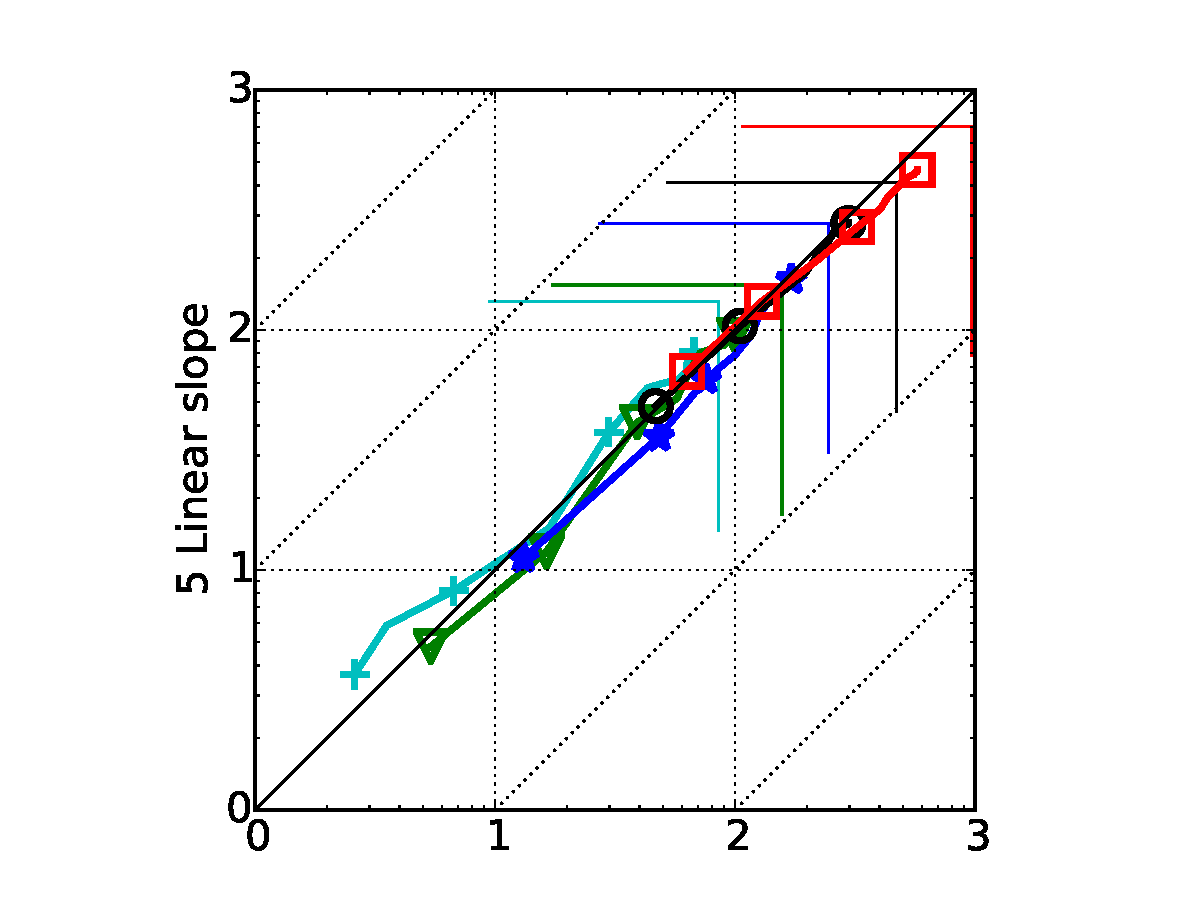
\includegraphics[width=0.25\textwidth, trim= 29mm 8.5mm 35mm 13mm, clip]{ppscatter_f005}&
    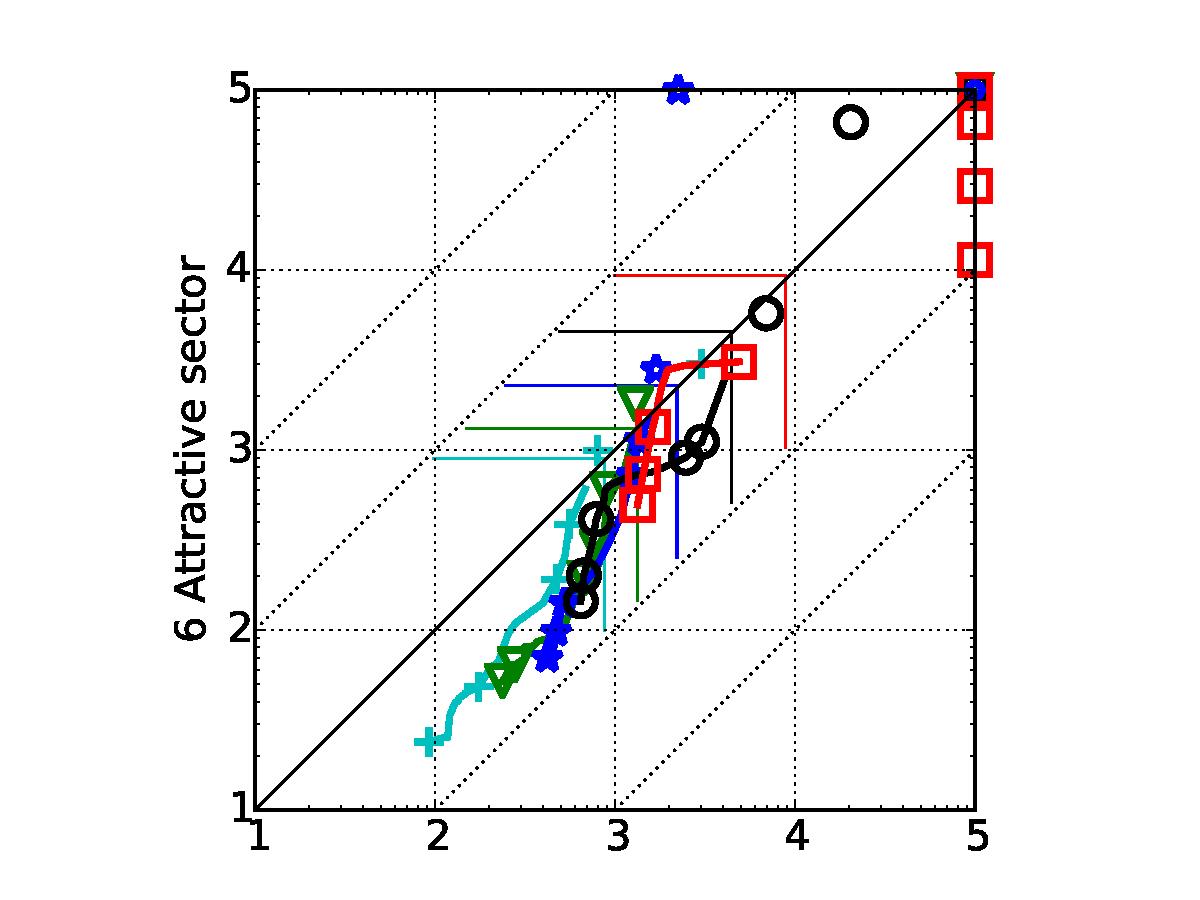
\includegraphics[width=0.25\textwidth, trim= 29mm 8.5mm 35mm 13mm, clip]{ppscatter_f006}&
    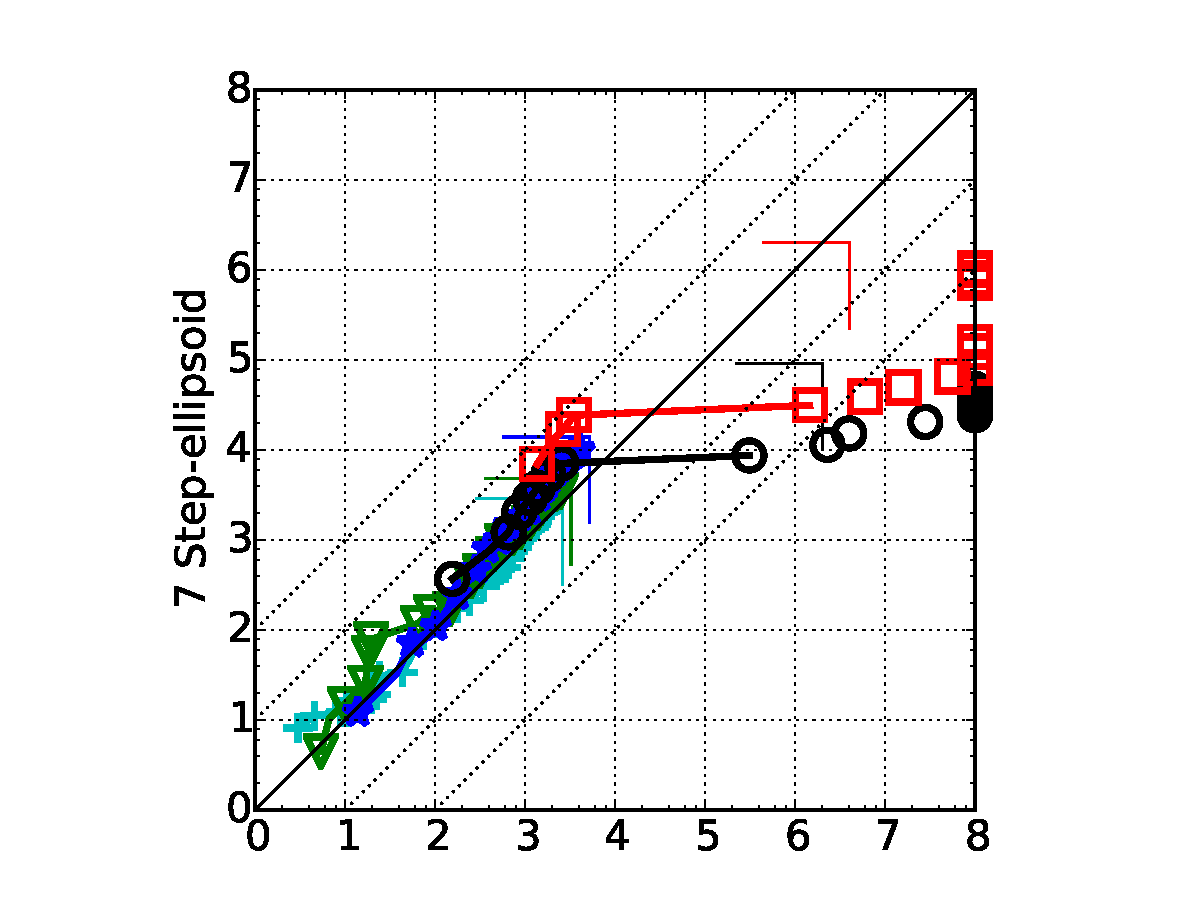
\includegraphics[width=0.25\textwidth, trim= 29mm 8.5mm 35mm 13mm, clip]{ppscatter_f007}&
    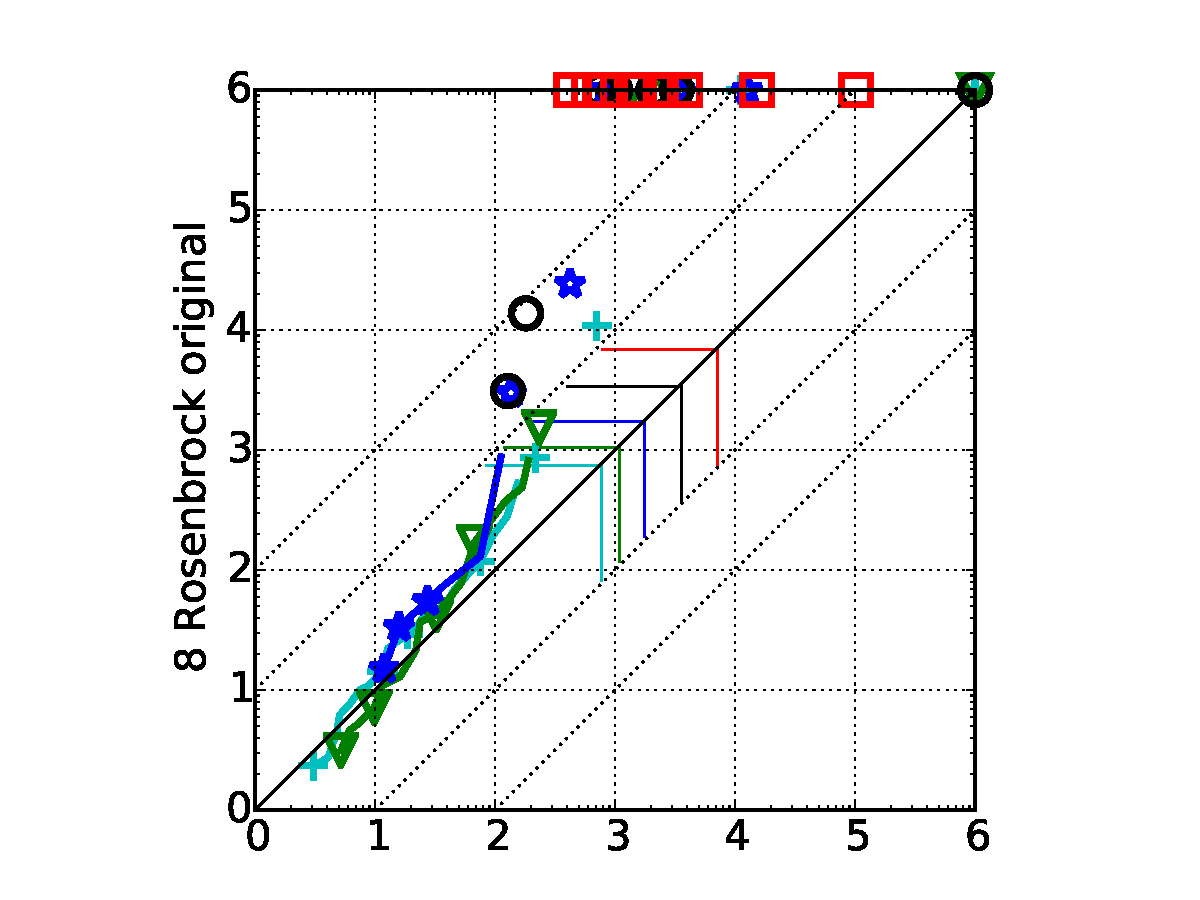
\includegraphics[width=0.25\textwidth, trim= 29mm 8.5mm 35mm 13mm, clip]{ppscatter_f008}\\
    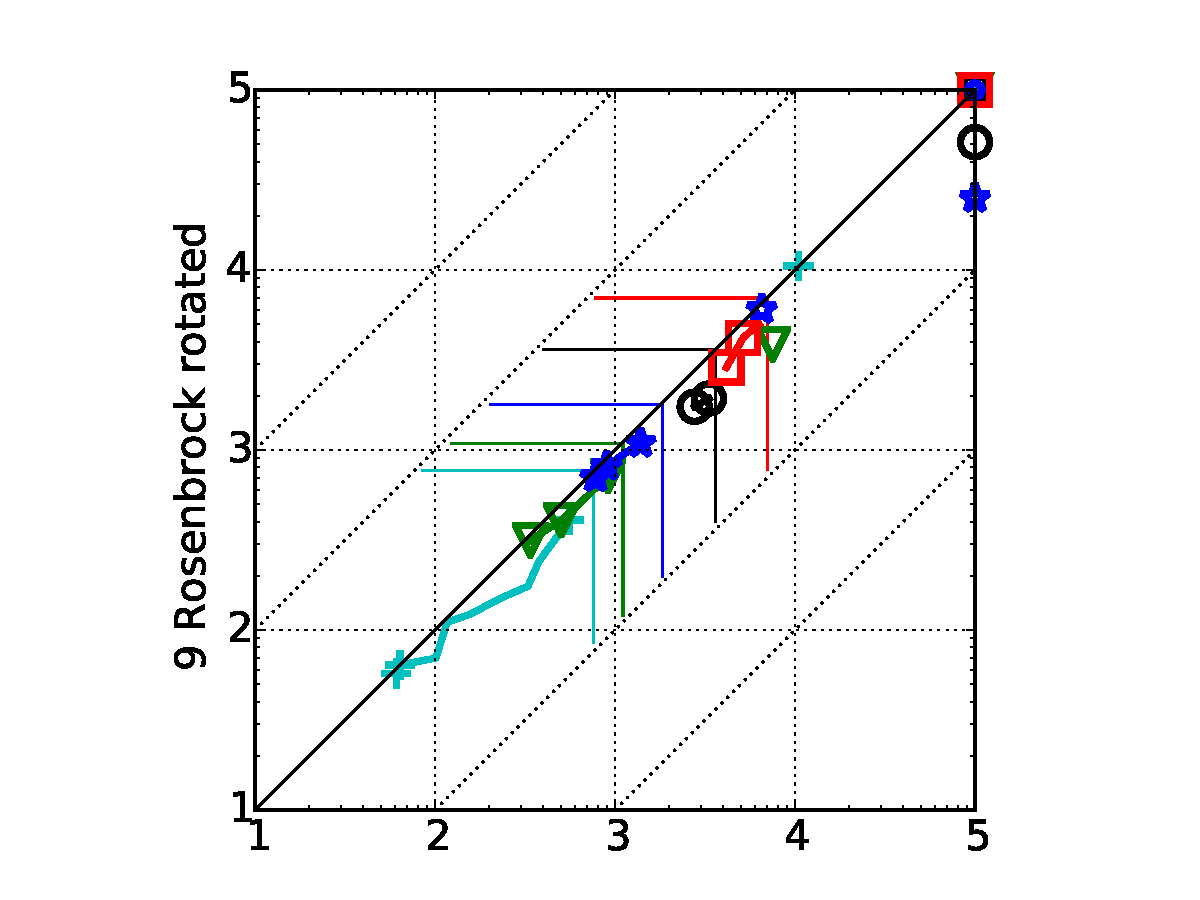
\includegraphics[width=0.25\textwidth, trim= 29mm 8.5mm 35mm 13mm, clip]{ppscatter_f009}&
    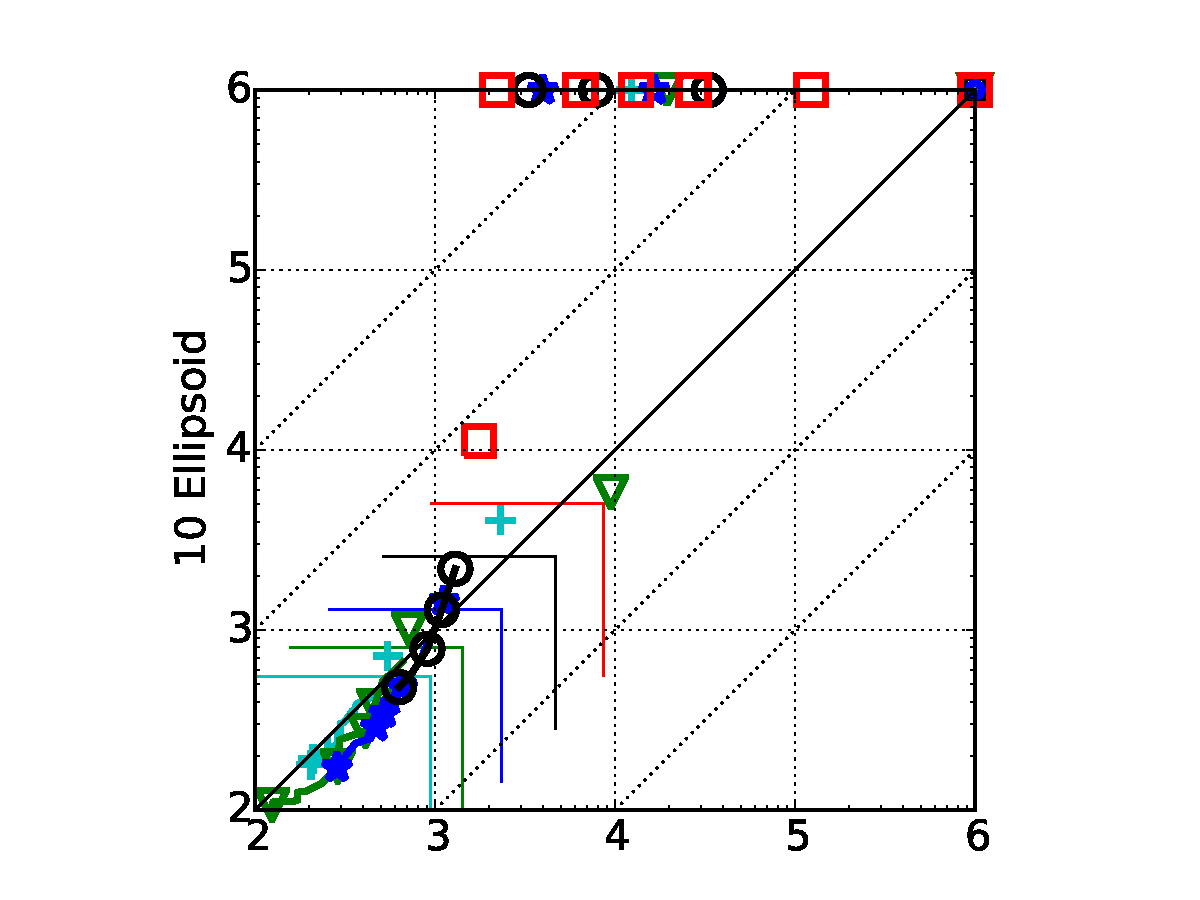
\includegraphics[width=0.25\textwidth, trim= 29mm 8.5mm 35mm 13mm, clip]{ppscatter_f010}&
    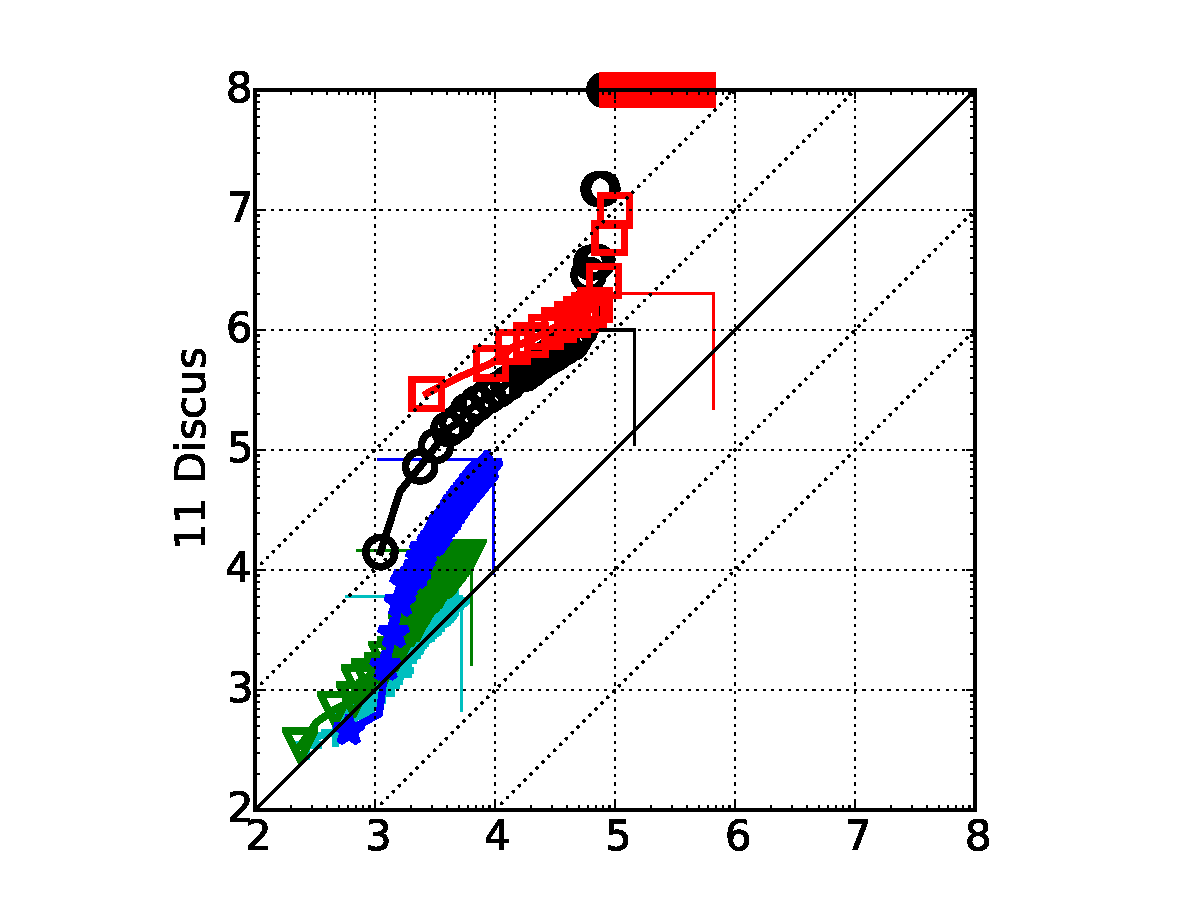
\includegraphics[width=0.25\textwidth, trim= 29mm 8.5mm 35mm 13mm, clip]{ppscatter_f011}&
    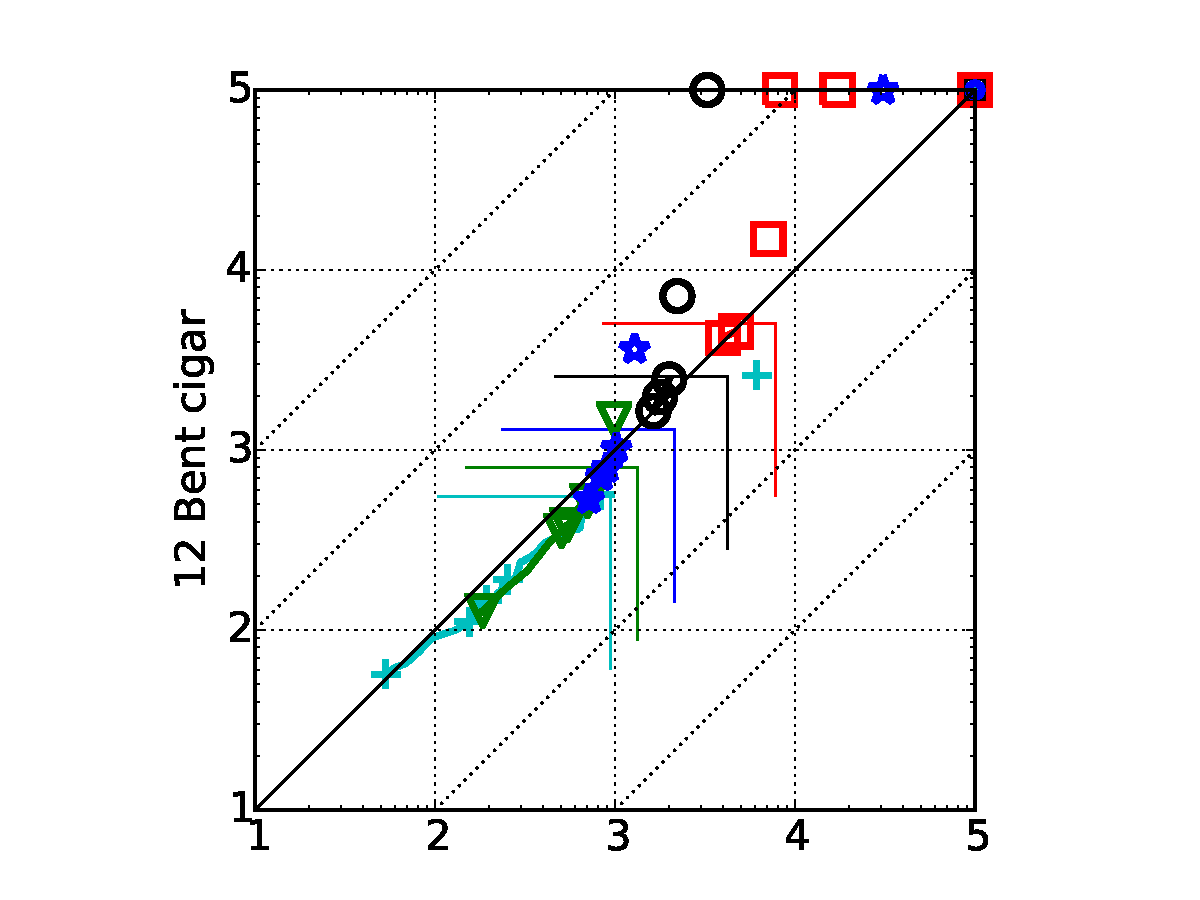
\includegraphics[width=0.25\textwidth, trim= 29mm 8.5mm 35mm 13mm, clip]{ppscatter_f012}\\
    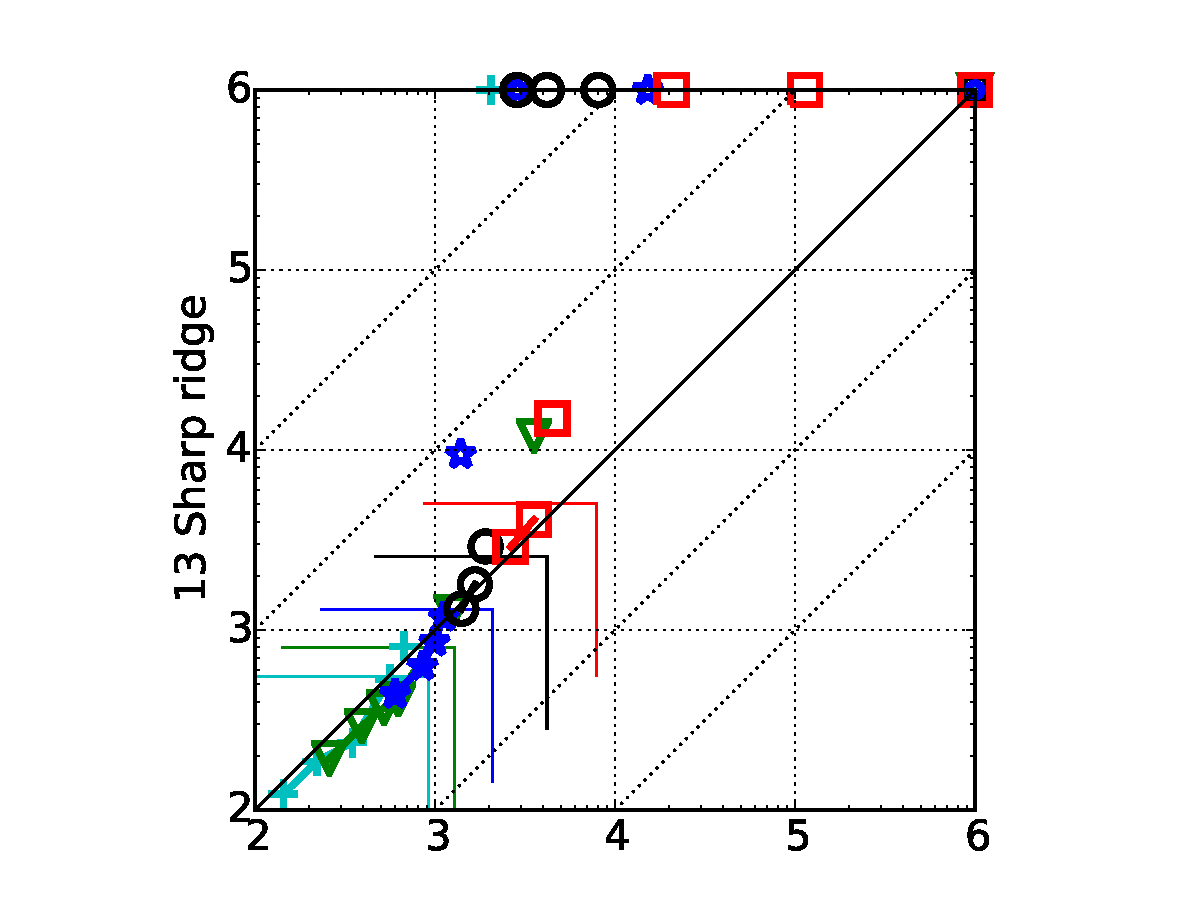
\includegraphics[width=0.25\textwidth, trim= 29mm 8.5mm 35mm 13mm, clip]{ppscatter_f013}&
    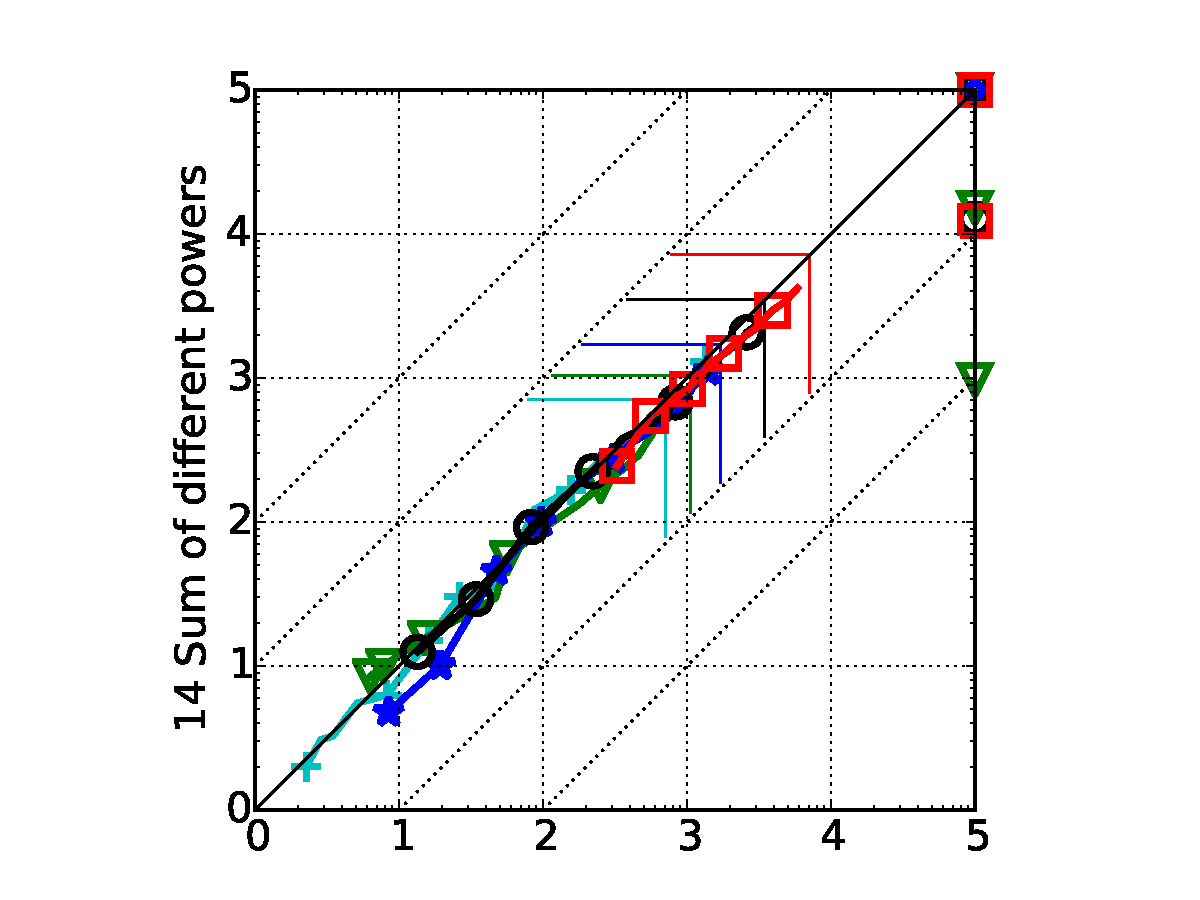
\includegraphics[width=0.25\textwidth, trim= 29mm 8.5mm 35mm 13mm, clip]{ppscatter_f014}&
    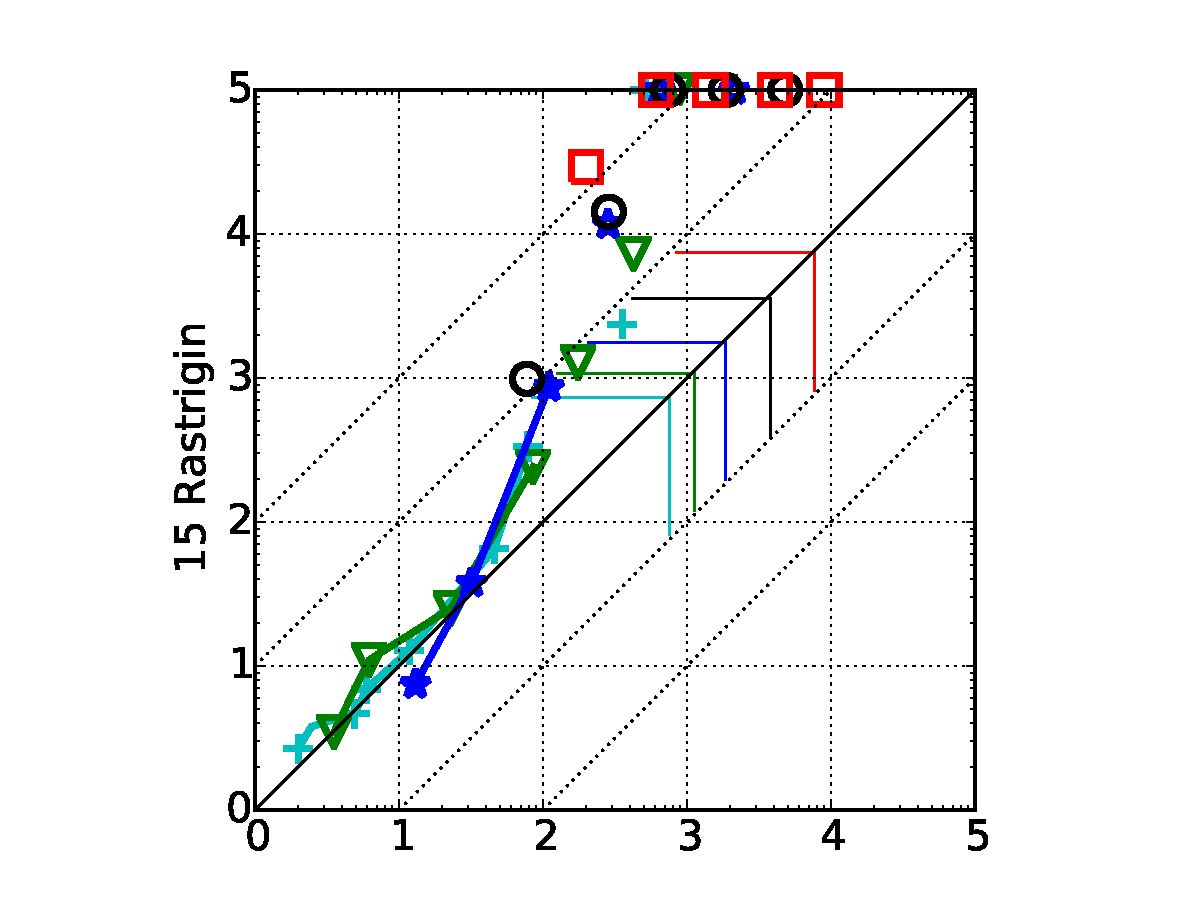
\includegraphics[width=0.25\textwidth, trim= 29mm 8.5mm 35mm 13mm, clip]{ppscatter_f015}&
    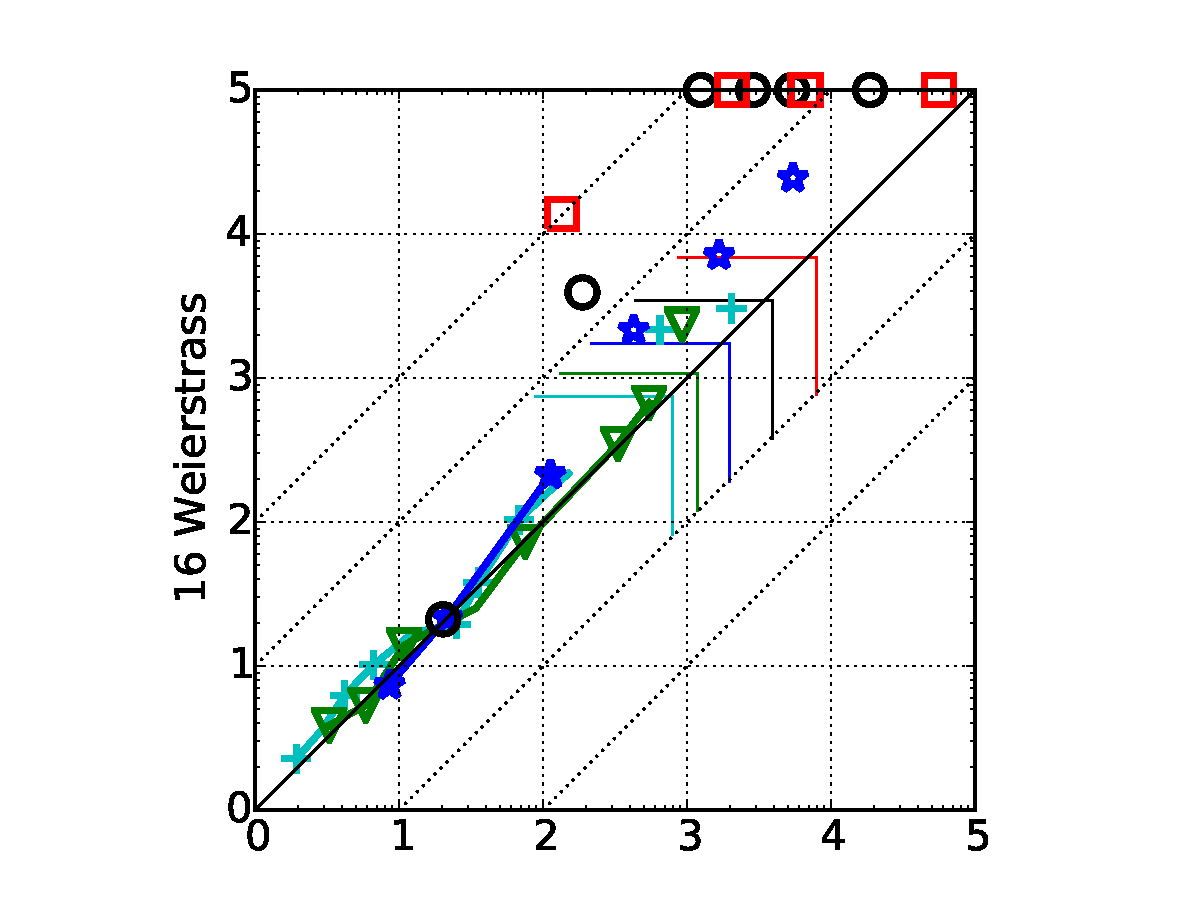
\includegraphics[width=0.25\textwidth, trim= 29mm 8.5mm 35mm 13mm, clip]{ppscatter_f016}\\
    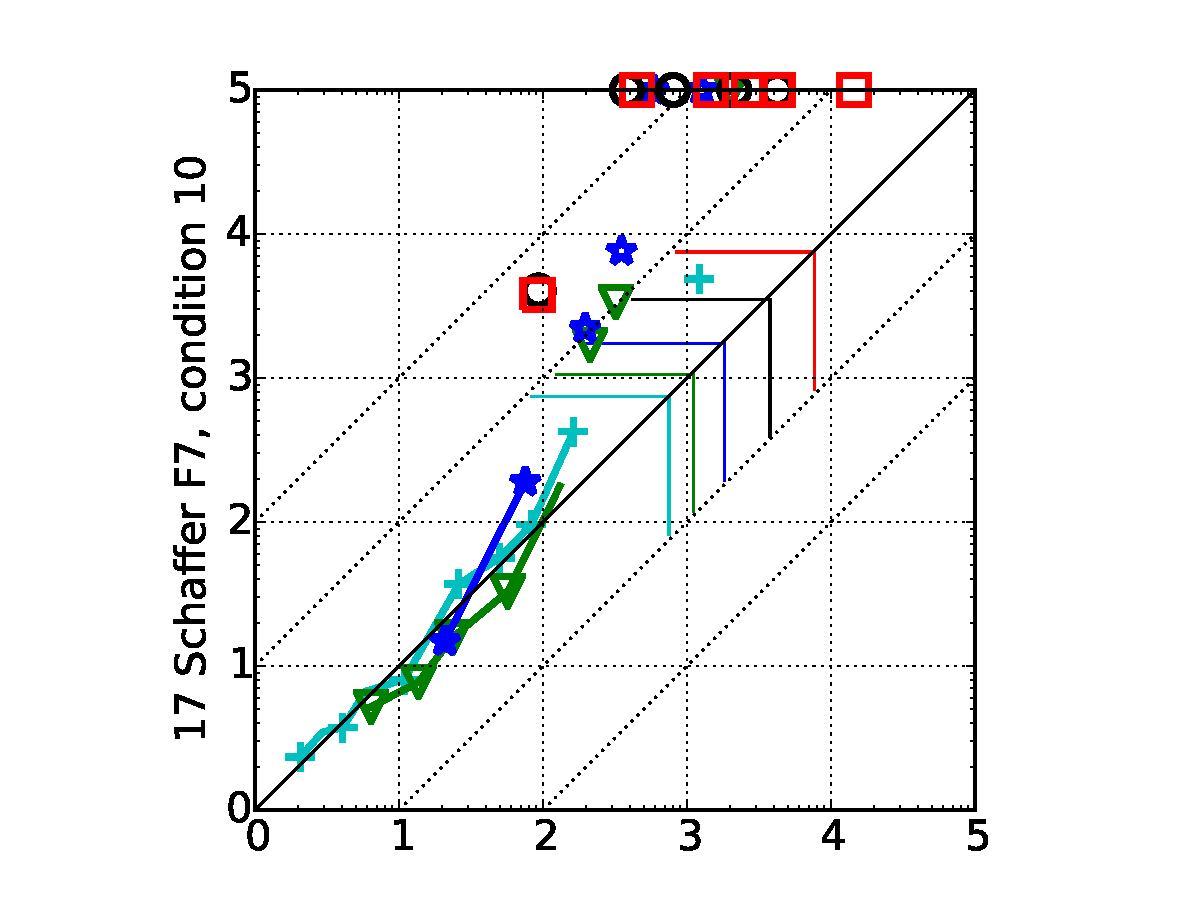
\includegraphics[width=0.25\textwidth, trim= 29mm 8.5mm 35mm 13mm, clip]{ppscatter_f017}&
    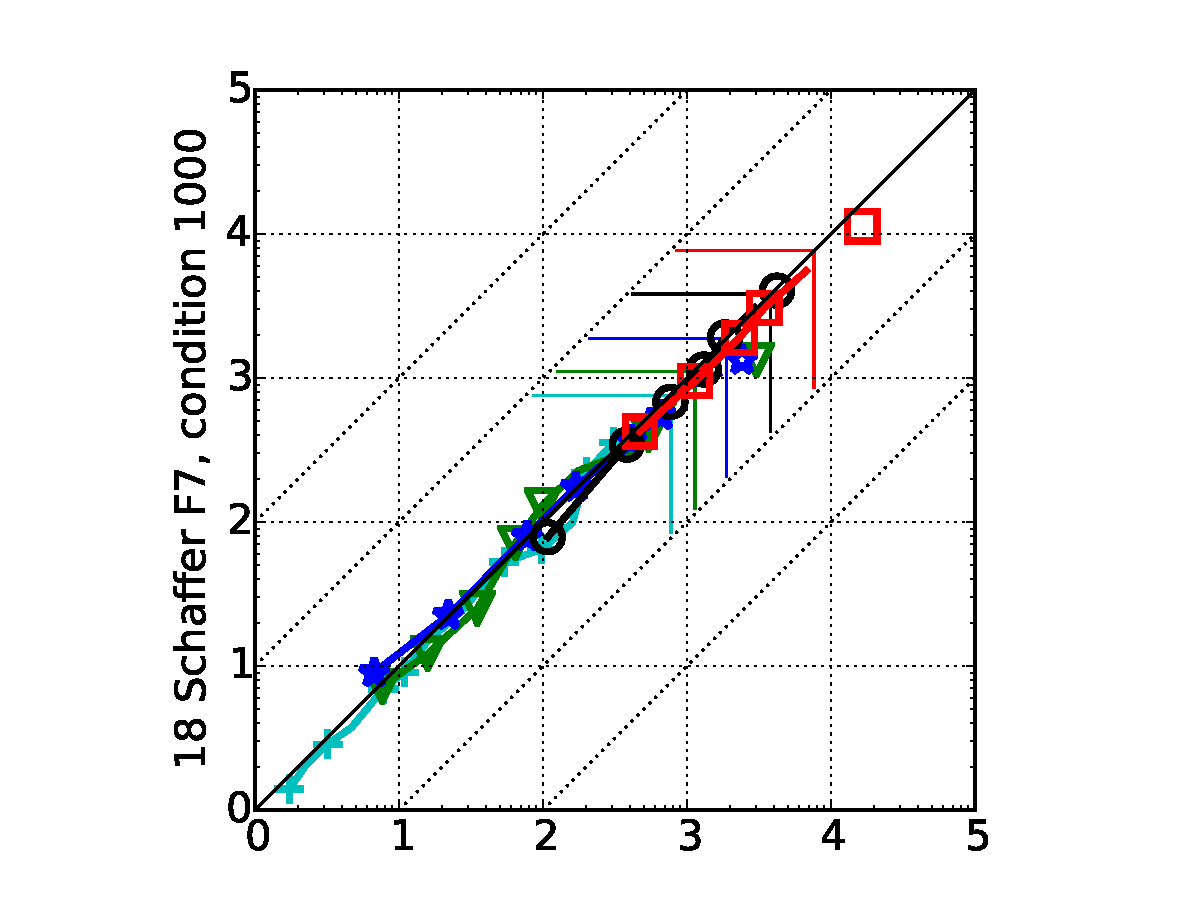
\includegraphics[width=0.25\textwidth, trim= 29mm 8.5mm 35mm 13mm, clip]{ppscatter_f018}&
    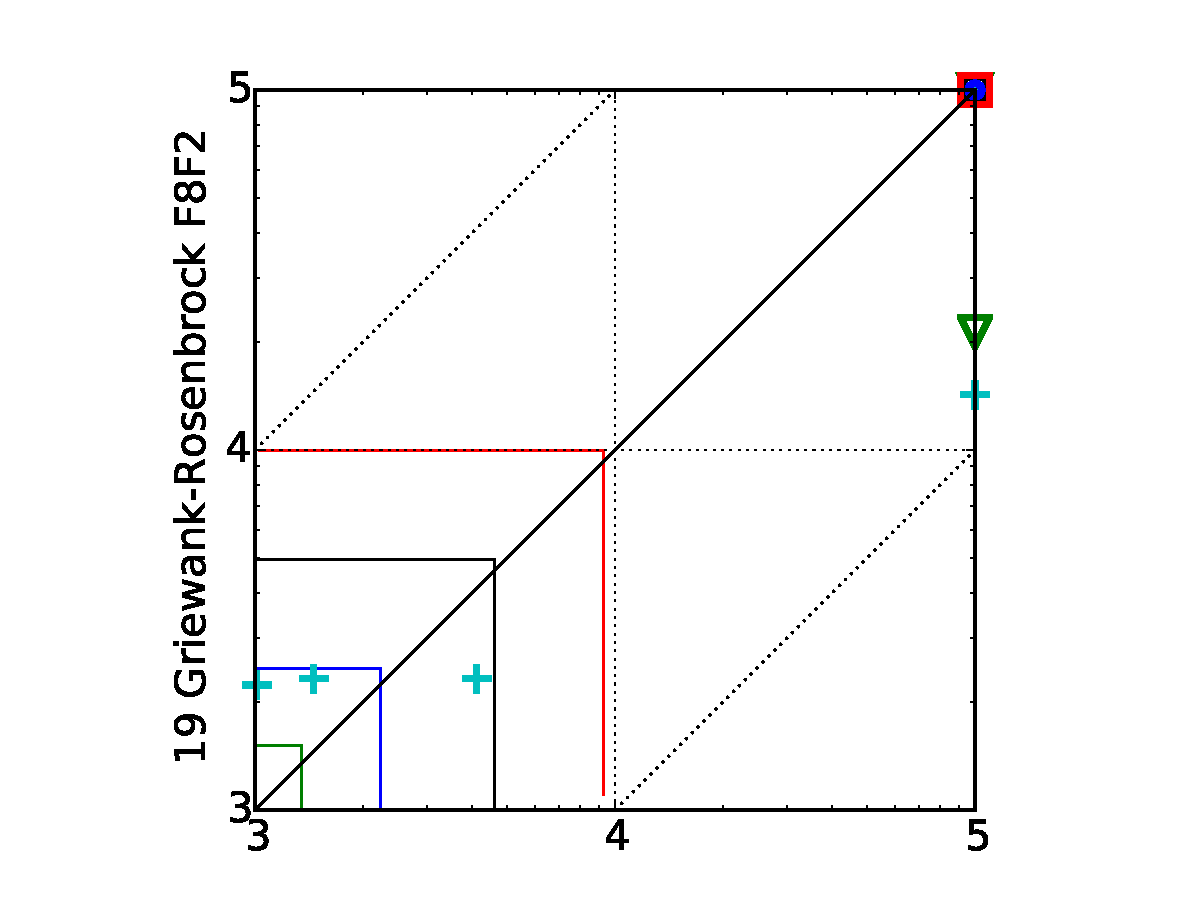
\includegraphics[width=0.25\textwidth, trim= 29mm 8.5mm 35mm 13mm, clip]{ppscatter_f019}&
    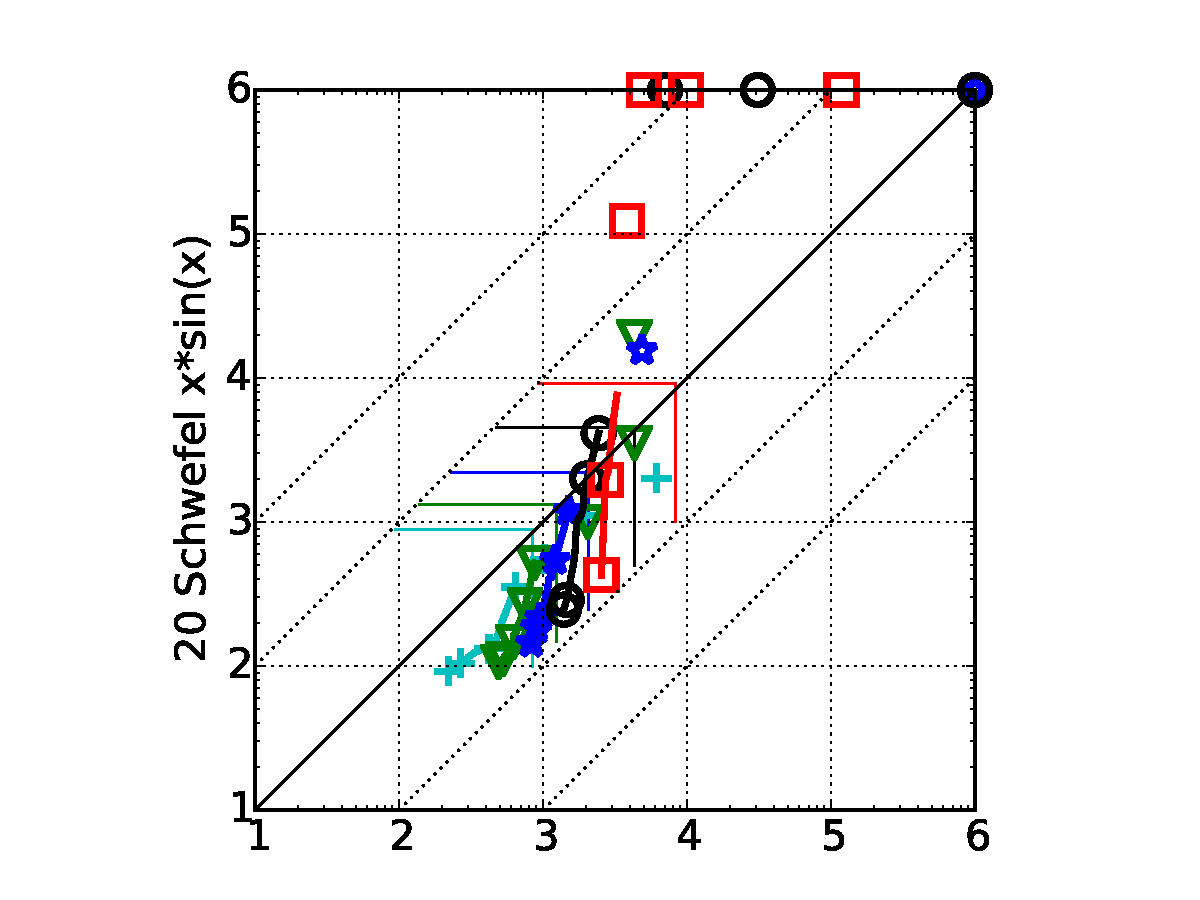
\includegraphics[width=0.25\textwidth, trim= 29mm 8.5mm 35mm 13mm, clip]{ppscatter_f020}\\
    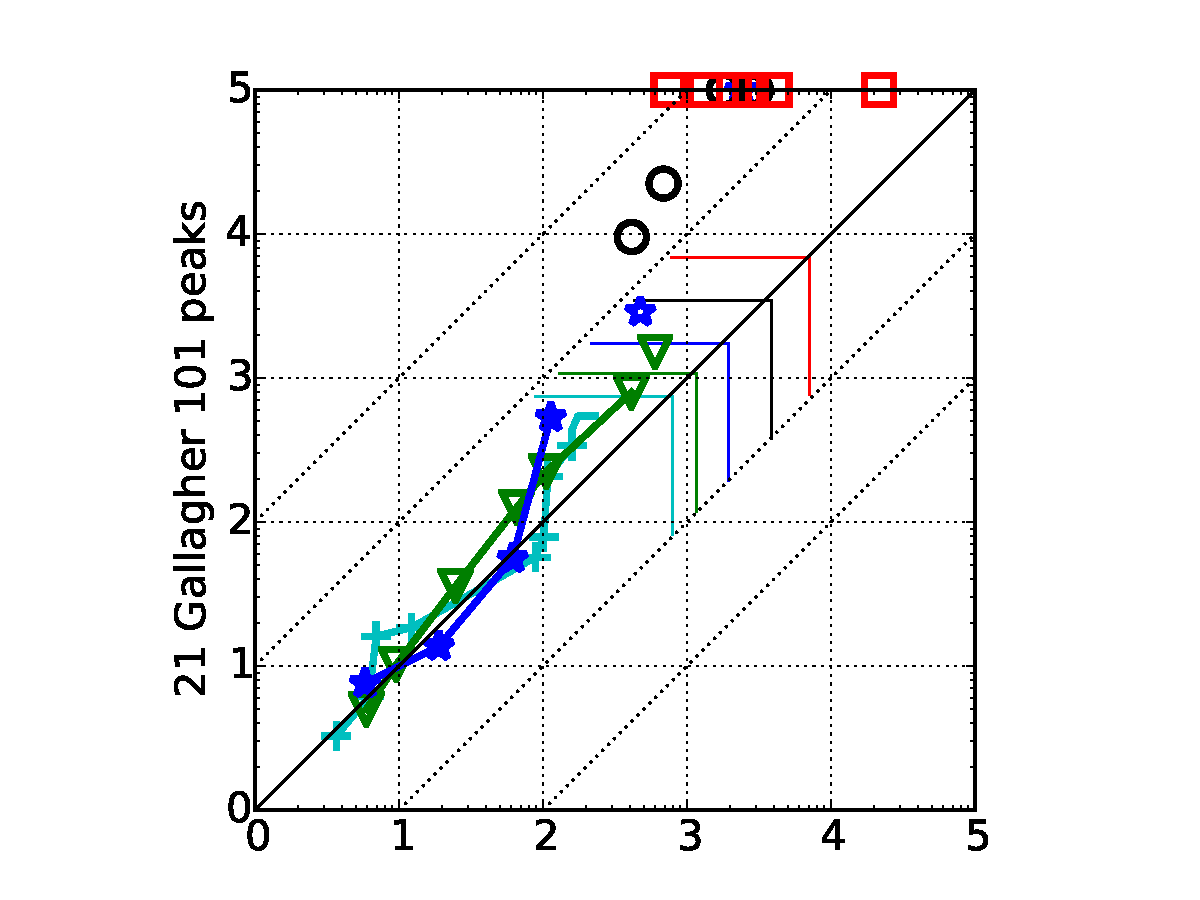
\includegraphics[width=0.25\textwidth, trim= 29mm 8.5mm 35mm 13mm, clip]{ppscatter_f021}&
    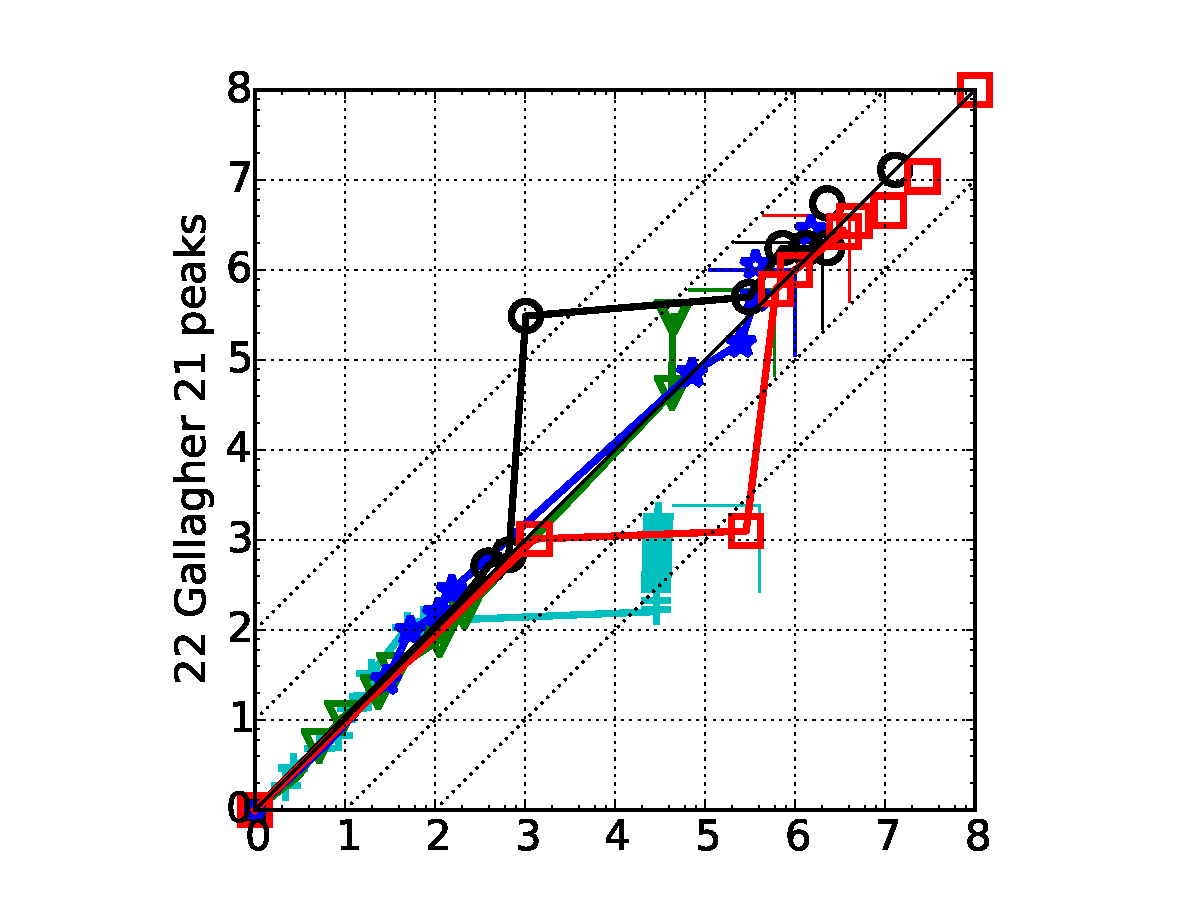
\includegraphics[width=0.25\textwidth, trim= 29mm 8.5mm 35mm 13mm, clip]{ppscatter_f022}&
    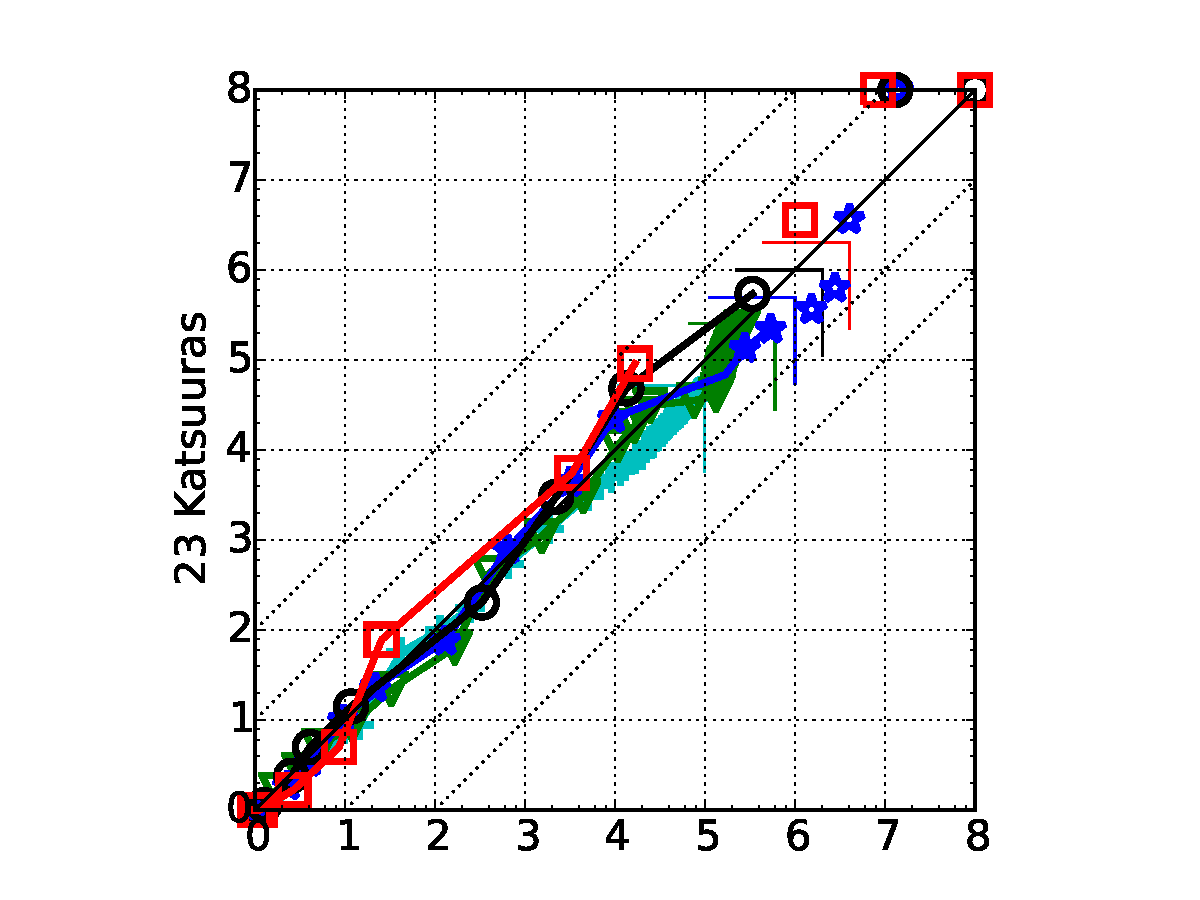
\includegraphics[width=0.25\textwidth, trim= 29mm 8.5mm 35mm 13mm, clip]{ppscatter_f023}&
    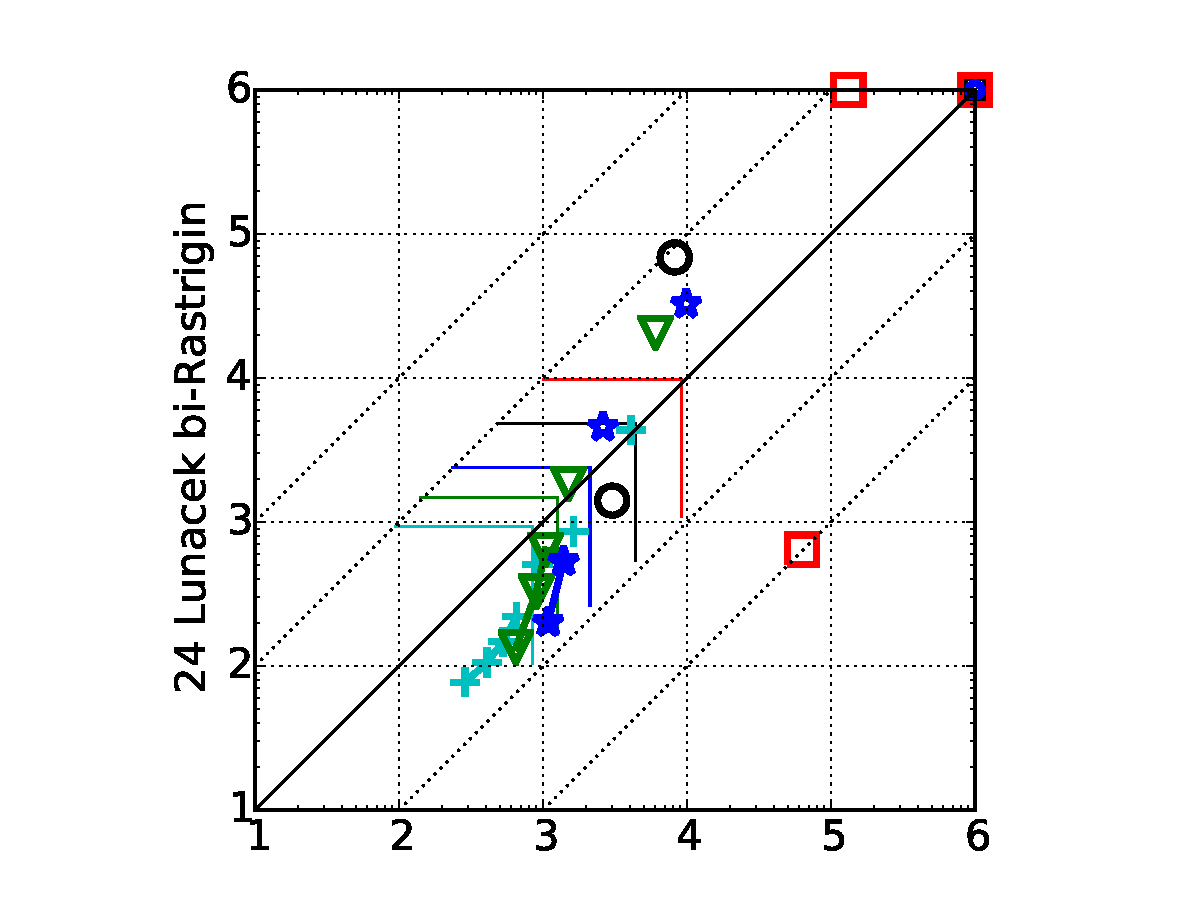
\includegraphics[width=0.25\textwidth, trim= 29mm 8.5mm 35mm 13mm, clip]{ppscatter_f024}
\end{tabular}
\bbobppscatterlegend{$f_1$--$f_{24}$}
\label{fig:scatterplots}
\end{figure}
%%%%%%%%%%%%%%%%%%%%%%%%%%%%%%%%%%%%%%%%%%%%%%%%%%%%%%%%%%%%%%%%%%%%%%%%%%%%%%%
%%%%%%%%%%%%%%%%%%%%%%%%%%%%%%%%%%%%%%%%%%%%%%%%%%%%%%%%%%%%%%%%%%%%%%%%%%%%%%%
\begin{figure}
\centering
\begin{tabular}{@{}c@{}c@{}c@{}c@{}}
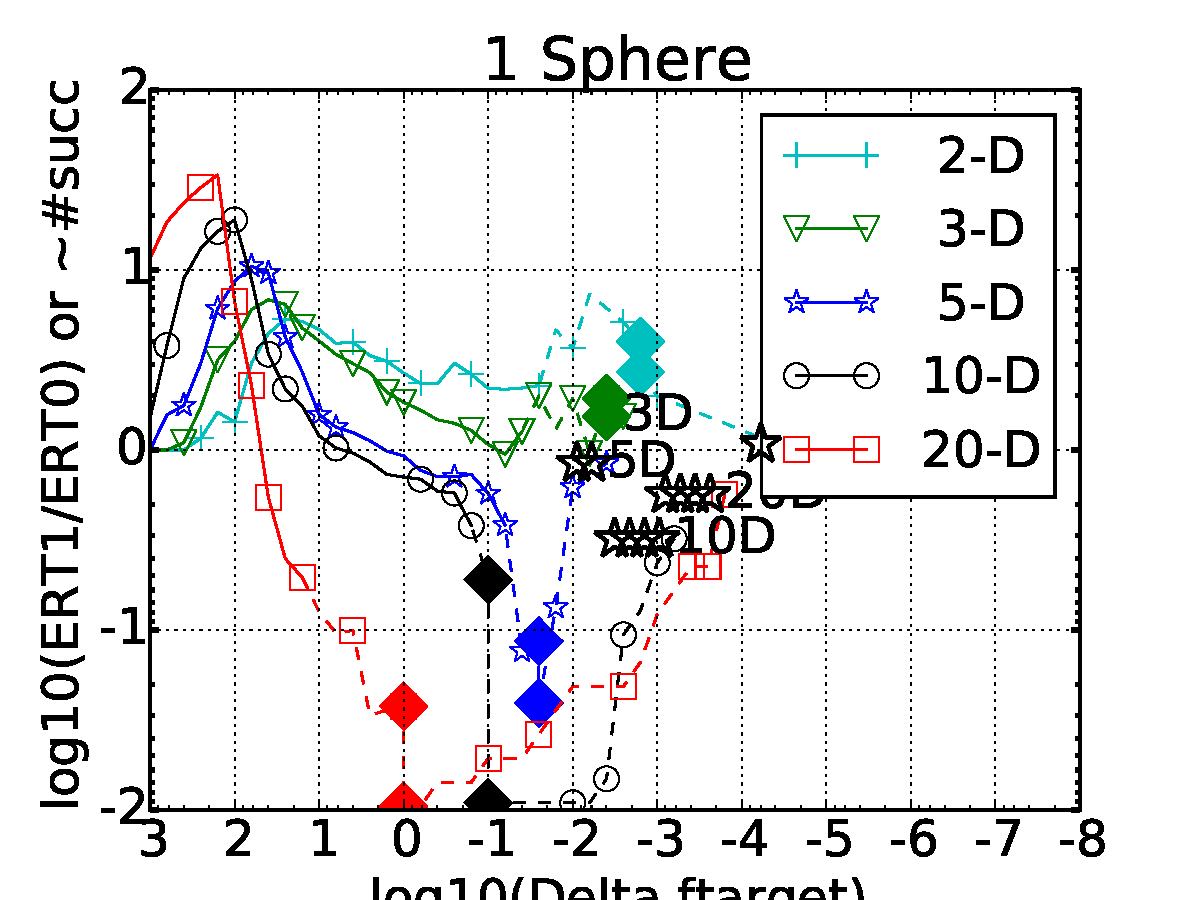
\includegraphics[width=0.253\textwidth, trim= 0.7cm 0.8cm 0.2cm 0.2cm, clip]{ppfig2_f001}&
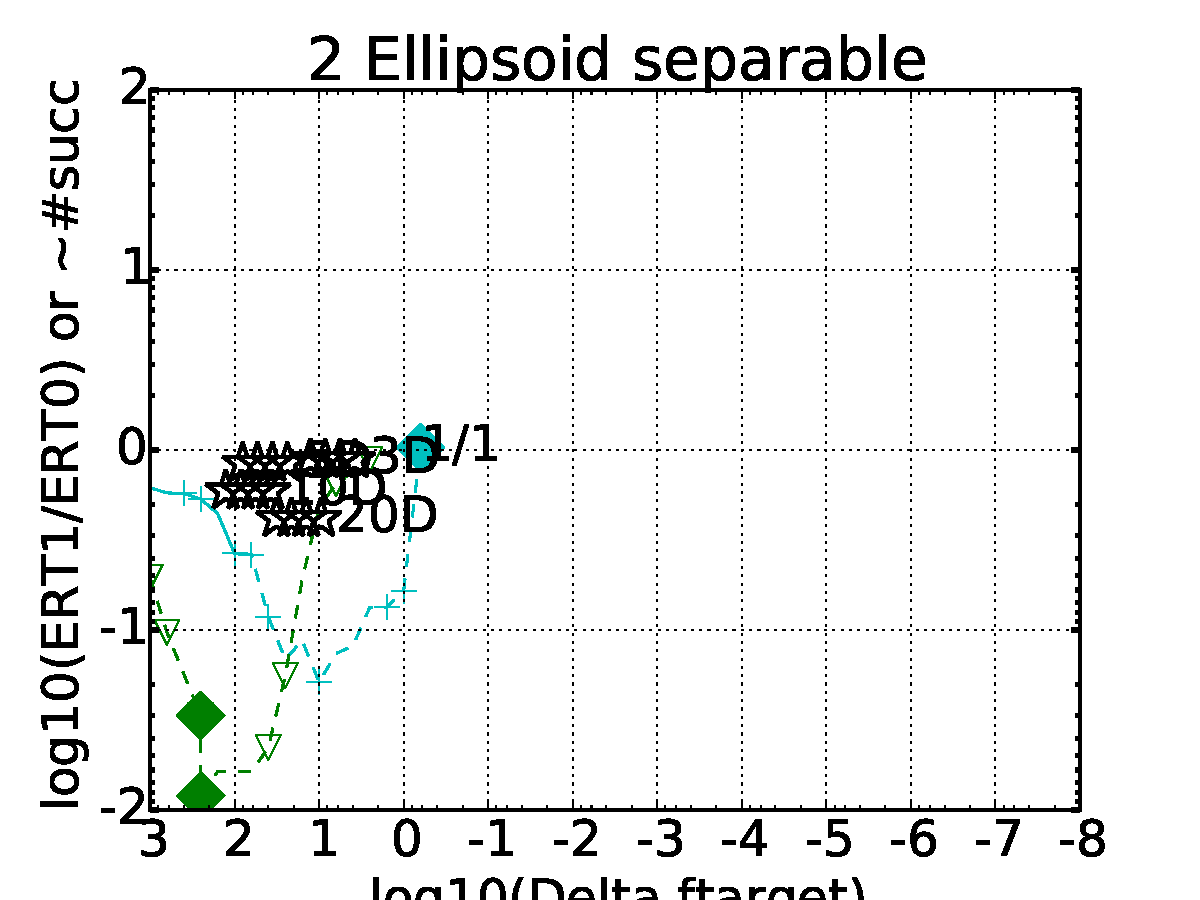
\includegraphics[width=0.238\textwidth, trim= 1.8cm 0.8cm 0.2cm 0.2cm, clip]{ppfig2_f002}&
\includegraphics[width=0.238\textwidth, trim= 1.8cm 0.8cm 0.2cm 0.2cm, clip]{ppfig2_f003}&
\includegraphics[width=0.238\textwidth, trim= 1.8cm 0.8cm 0.2cm 0.2cm, clip]{ppfig2_f004}\\
\includegraphics[width=0.253\textwidth, trim= 0.7cm 0.8cm 0.2cm 0.2cm, clip]{ppfig2_f005}&
\includegraphics[width=0.238\textwidth, trim= 1.8cm 0.8cm 0.2cm 0.2cm, clip]{ppfig2_f006}&
\includegraphics[width=0.238\textwidth, trim= 1.8cm 0.8cm 0.2cm 0.2cm, clip]{ppfig2_f007}&
\includegraphics[width=0.238\textwidth, trim= 1.8cm 0.8cm 0.2cm 0.2cm, clip]{ppfig2_f008}\\
\includegraphics[width=0.253\textwidth, trim= 0.7cm 0.8cm 0.2cm 0.2cm, clip]{ppfig2_f009}&
\includegraphics[width=0.238\textwidth, trim= 1.8cm 0.8cm 0.2cm 0.2cm, clip]{ppfig2_f010}&
\includegraphics[width=0.238\textwidth, trim= 1.8cm 0.8cm 0.2cm 0.2cm, clip]{ppfig2_f011}&
\includegraphics[width=0.238\textwidth, trim= 1.8cm 0.8cm 0.2cm 0.2cm, clip]{ppfig2_f012}\\
\includegraphics[width=0.253\textwidth, trim= 0.7cm 0.8cm 0.2cm 0.2cm, clip]{ppfig2_f013}&
\includegraphics[width=0.238\textwidth, trim= 1.8cm 0.8cm 0.2cm 0.2cm, clip]{ppfig2_f014}&
\includegraphics[width=0.238\textwidth, trim= 1.8cm 0.8cm 0.2cm 0.2cm, clip]{ppfig2_f015}&
\includegraphics[width=0.238\textwidth, trim= 1.8cm 0.8cm 0.2cm 0.2cm, clip]{ppfig2_f016}\\
\includegraphics[width=0.253\textwidth, trim= 0.7cm 0.8cm 0.2cm 0.2cm, clip]{ppfig2_f017}&
\includegraphics[width=0.238\textwidth, trim= 1.8cm 0.8cm 0.2cm 0.2cm, clip]{ppfig2_f018}&
\includegraphics[width=0.238\textwidth, trim= 1.8cm 0.8cm 0.2cm 0.2cm, clip]{ppfig2_f019}&
\includegraphics[width=0.238\textwidth, trim= 1.8cm 0.8cm 0.2cm 0.2cm, clip]{ppfig2_f020}\\
\includegraphics[width=0.253\textwidth, trim= 0.7cm 0.0cm 0.2cm 0.2cm, clip]{ppfig2_f021}&
\includegraphics[width=0.238\textwidth, trim= 1.8cm 0.0cm 0.2cm 0.2cm, clip]{ppfig2_f022}&
\includegraphics[width=0.238\textwidth, trim= 1.8cm 0.0cm 0.2cm 0.2cm, clip]{ppfig2_f023}&
\includegraphics[width=0.238\textwidth, trim= 1.8cm 0.0cm 0.2cm 0.2cm, clip]{ppfig2_f024}
\end{tabular}
\vspace*{-0.2cm}
\caption{\label{fig:ERTratiographs}Ratio of \ERT\ for \algorithmB\ over \ERT\ for
\algorithmA\ versus $\log_{10}(\Df)$ in
  2:{\color{cyan}+},
  3:{\color{green!45!black}$\triangledown$},
  5:{\color{blue}$\star$}, 
 10:$\circ$, 
 20:{\color{red}$\Box$}, 
 40-D:{\color{magenta}$\Diamond$}.
% cyan:2, green:3, blue:5, black:10, red:20, purple:40. 
Ratios $<10^0$ indicate an advantage of \algorithmB, smaller
values are always better. The line becomes dashed when for any algorithm the \ERT\ exceeds thrice the median
of the trial-wise overall number of $f$-evaluations for the same algorithm on this function.
Filled symbols indicate the best achieved $\Df$-value of one algorithm (\ERT\ is undefined to the right).
The dashed line continues as the fraction of successful trials of the other
algorithm, where 0 means 0\% and the y-axis limits mean 100\%, values below
zero for \algorithmB. The line ends when no algorithm reaches $\Df$ anymore. 
The number of successful trials is given, only if it was in $\{1\dots9\}$ for
\algorithmB\ (1$^{\textrm{st}}$ number) and non-zero for \algorithmA\ (2$^{\textrm{nd}}$ number).
Results are significant with $p=0.05$ for one star and $p=10^{-\#\star}$
otherwise, with Bonferroni correction within each figure.}
\end{figure}
%%%%%%%%%%%%%%%%%%%%%%%%%%%%%%%%%%%%%%%%%%%%%%%%%%%%%%%%%%%%%%%%%%%%%%%%%%%%%%%%%%%%%%%%%%%%%%%%%%%%%%%%%%%%%%%%%%%%%%%%%%%%%%%%%%%%%%%%%%%%%%%%%%%%%%%%%%%%%%
%%%%%%%%%%%%%%%%%%%%%%%%%%%%%%%%%%%%%%%%%%%%%%%%%%%%%%%%%%%%%%%%%%%%%%%%%%%%%%%
\begin{figure}[htbp!]
\centering
\begin{tabular}{@{}c@{}c@{}}
\rot[5]{all functions}\includegraphics[width=0.528\textwidth,trim=0 0mm 16mm 11mm, clip]{pprldistr_05D_noiselessall} &
\includegraphics[width=0.46\textwidth,trim=24mm 0mm 16mm 11mm, clip]{pplogabs_05D_noiselessall}\\
\rot[5]{all functions}\includegraphics[width=0.528\textwidth,trim=0 0mm 16mm 11mm, clip]{pprldistr_20D_noiselessall} &
\includegraphics[width=0.46\textwidth,trim=24mm 0mm 16mm 11mm, clip]{pplogabs_20D_noiselessall}
\end{tabular}
\caption{\label{fig:RLDs05Da}Noiseless functions 5-D (top) and 20-D (bottom).
Left:
Empirical Cumulative Distribution Function (ECDF) of the running time (number
of function evaluations) for \algorithmB\ ($\circ$) and \algorithmA\ ($\triangledown$), divided by
search space dimension $D$, to fall below $\fopt+\Df$ with $\Df = 10^k$ where
$k$ is the value in the legend. The vertical black lines indicate the maximum
number of function evaluations. Light beige lines in the background show ECDFs
for target value $10^{-8}$ of all algorithms benchmarked during BBOB 2009.
Right subplots: ECDF of \ERT\ of \algorithmB\ over \ERT\ of \algorithmA\ for
different $\Df$.
}
\end{figure}
%%%%%%%%%%%%%%%%%%%%%%%%%%%%%%%%%%%%%%%%%%%%%%%%%%%%%%%%%%%%%%%%%%%%%%%%%%%%%%%
\begin{figure}[htbp!]
\centering
\begin{tabular}{@{}c@{}c@{}}
\rot[2.5]{separable fcts}
\includegraphics[width=0.41\textwidth,trim=0 7.5mm 16mm 11mm, clip]{pprldistr_05D_separ} &
\includegraphics[width=0.3579\textwidth,trim=24mm 7.5mm 16mm 11mm, clip]{pplogabs_05D_separ}
\\[-1ex]
\rot[1.3]{misc.\ moderate fcts}
\includegraphics[width=0.41\textwidth,trim=0 7.5mm 16mm 11mm, clip]{pprldistr_05D_lcond} &
\includegraphics[width=0.3579\textwidth,trim=24mm 7.5mm 16mm 11mm, clip]{pplogabs_05D_lcond}
\\[-1ex]
\rot[1.1]{ill-conditioned fcts}
\includegraphics[width=0.41\textwidth,trim=0 7.5mm 16mm 11mm, clip]{pprldistr_05D_hcond} &
\includegraphics[width=0.3579\textwidth,trim=24mm 7.5mm 16mm 11mm, clip]{pplogabs_05D_hcond}
\\[-1ex]
\rot[1.7]{multi-modal fcts}
\includegraphics[width=0.41\textwidth,trim=0 7.5mm 16mm 11mm, clip]{pprldistr_05D_multi} &
\includegraphics[width=0.3579\textwidth,trim=24mm 7.5mm 16mm 11mm, clip]{pplogabs_05D_multi}
\\[-1ex]
\rot[1.5]{weak structure fcts}
\includegraphics[width=0.41\textwidth,trim=0 0mm 16mm 11mm, clip]{pprldistr_05D_mult2} &
\includegraphics[width=0.3579\textwidth,trim=24mm 0mm 16mm 11mm, clip]{pplogabs_05D_mult2}
\end{tabular}
\vspace*{-0.5ex}
\caption{\label{fig:RLDs05Db}Subgroups of functions 5-D. See caption of Figure~\ref{fig:RLDs05Da}.}
\end{figure}
%%%%%%%%%%%%%%%%%%%%%%%%%%%%%%%%%%%%%%%%%%%%%%%%%%%%%%%%%%%%%%%%%%%%%%%%%%%%%%%

%%%%%%%%%%%%%%%%%%%%%%%%%%%%%%%%%%%%%%%%%%%%%%%%%%%%%%%%%%%%%%%%%%%%%%%%%%%%%%%
\begin{figure}[htbp!]
\centering
\begin{tabular}{@{}c@{}c@{}}
\rot[2.5]{separable fcts}
\includegraphics[width=0.41\textwidth,trim=0 7.5mm 16mm 11mm, clip]{pprldistr_20D_separ} &
\includegraphics[width=0.3579\textwidth,trim=24mm 7.5mm 16mm 11mm, clip]{pplogabs_20D_separ}
\\[-1ex]
\rot[1.3]{misc.\ moderate fcts}
\includegraphics[width=0.41\textwidth,trim=0 7.5mm 16mm 11mm, clip]{pprldistr_20D_lcond} &
\includegraphics[width=0.3579\textwidth,trim=24mm 7.5mm 16mm 11mm, clip]{pplogabs_20D_lcond}
\\[-1ex]
\rot[1.1]{ill-conditioned fcts}
\includegraphics[width=0.41\textwidth,trim=0 7.5mm 16mm 11mm, clip]{pprldistr_20D_hcond} &
\includegraphics[width=0.3579\textwidth,trim=24mm 7.5mm 16mm 11mm, clip]{pplogabs_20D_hcond}
\\[-1ex]
\rot[1.7]{multi-modal fcts}
\includegraphics[width=0.41\textwidth,trim=0 7.5mm 16mm 11mm, clip]{pprldistr_20D_multi} &
\includegraphics[width=0.3579\textwidth,trim=24mm 7.5mm 16mm 11mm, clip]{pplogabs_20D_multi}
\\[-1ex]
\rot[1.5]{weak structure fcts}
\includegraphics[width=0.41\textwidth,trim=0 0mm 16mm 11mm, clip]{pprldistr_20D_mult2} &
\includegraphics[width=0.3579\textwidth,trim=24mm 0mm 16mm 11mm, clip]{pplogabs_20D_mult2}
\end{tabular}
\vspace*{-0.5ex}
\caption{\label{fig:RLDs20Db}Subgroups of functions 20-D. See caption of Figure~\ref{fig:RLDs05Da}.}
\end{figure}
%%%%%%%%%%%%%%%%%%%%%%%%%%%%%%%%%%%%%%%%%%%%%%%%%%%%%%%%%%%%%%%%%%%%%%%%%%%%%%%
%%%%%%%%%%%%%%%%%%%%%%%%%%%%%%%%%%%%%%%%%%%%%%%%%%%%%%%%%%%%%%%%%%%%%%%%%%%%%%%
% you can define the commands \algorithmAshort and \algorithmBshort here to override
% the definition in the pptable2_xxD_xxxx.tex files for the following tables
% \newcommand{\algorithmAshort}{XX1}
% \newcommand{\algorithmBshort}{XX2}
%%%%%%%%%%%%%%%%%%%%%%%%%%%%%%%%%%%%%%%%%%%%%%%%%%%%%%%%%%%%%%%%%%%%%%%%%%%%%%%
\begin{table}
\centering
\caption{\label{tab:ERTs05D} \bbobpptablestwolegend{48} Results for 5D.}
%\ERT\ and half-interquantile range (90\% -- 10\%)
%divided by the best \ERT\ measured during BBOB 2009 for different $\Df$ values
%for functions $f_1$--$f_{24}$ in 5-D where 0:\:\algorithmAshort\ is \algorithmA\ %and
%1:\:\algorithmBshort\ is \algorithmB}
\tiny
\input{\bbobdatapath pptable2_05D_noiselessall}
\end{table}
%%%%%%%%%%%%%%%%%%%%%%%%%%%%%%%%%%%%%%%%%%%%%%%%%%%%%%%%%%%%%%%%%%%%%%%%%%%%%%%
%%%%%%%%%%%%%%%%%%%%%%%%%%%%%%%%%%%%%%%%%%%%%%%%%%%%%%%%%%%%%%%%%%%%%%%%%%%%%%%
%%%%%%%%%%%%%%%%%%%%%%%%%%%%%%%%%%%%%%%%%%%%%%%%%%%%%%%%%%%%%%%%%%%%%%%%%%%%%%%
\begin{table}
\centering
\caption{\label{tab:ERTs20D}\bbobpptablestwolegend{48} Results for 20D.
%\ERT\ and half-interquantile range (90\% -- 10\%)
%divided by the best \ERT\ measured during BBOB 2009 for different $\Df$ values
%for functions $f_1$--$f_{24}$ in 20-D where 0:\:\algorithmAshort\ is \algorithmA\% and
%1:\:\algorithmBshort\ is \algorithmB
}
\tiny
\input{\bbobdatapath pptable2_20D_noiselessall}
\end{table}
%%%%%%%%%%%%%%%%%%%%%%%%%%%%%%%%%%%%%%%%%%%%%%%%%%%%%%%%%%%%%%%%%%%%%%%%%%%%%%%
% The following two commands are all you need in the
% initial runs of your .tex file to
% produce the bibliography for the citations in your paper.
\bibliographystyle{abbrv}
\bibliography{bbob}  % bbob.bib is the name of the Bibliography in this case
% You must have a proper ".bib" file
%  and remember to run:
% latex bibtex latex latex
% to resolve all references
\end{document}

